\documentclass[onecolumn,draftcls]{IEEEtran}
\usepackage{epsf,graphicx,color,epstopdf}
\usepackage{lineno}
\usepackage{setspace}
\usepackage{hyperref}
\usepackage{soul}

\newcommand{\exvivo}{\textit{ex vivo }}
\newcommand{\invivo}{\textit{in vivo }}
\newcommand{\invitro}{\textit{in vitro }}
\newcommand{\insitu}{\textit{in situ }}
\newcommand{\degree}{$^\circ$}
\newcommand{\isppa}{$I_\textrm{sppa}$}
\newcommand{\etal}{\textit{et al.}}
\newcommand{\attenunit}{dB$\cdot$cm$^{-1}$MHz$^{-1}$}

% load in data variables written in Matlab scripts / functions
\newcommand{\totalApexBaseRsq}{0.12}
\newcommand{\centralApexBaseRsq}{0.48}
\newcommand{\totalLatLatRsq}{0.39}
\newcommand{\centralLatLatRsq}{0.58}
\newcommand{\totalAntPostRsq}{0.35}
\newcommand{\centralAntPostRsq}{0.24}

\newcommand{\ARFImrTotalLatLatMeanPct}{18.4}
\newcommand{\ARFImrCentralLatLatMeanPct}{21.5}
\newcommand{\ARFImrTotalLatLatStdPct}{13.9}
\newcommand{\ARFImrCentralLatLatStdPct}{14.3}
\newcommand{\ARFImrTotalAntPostMeanPct}{7.4}
\newcommand{\ARFImrCentralAntPostMeanPct}{-0.6}
\newcommand{\ARFImrTotalAntPostStdPct}{17.6}
\newcommand{\ARFImrCentralAntPostStdPct}{20.8}
\newcommand{\ARFImrTotalApexBaseMeanPct}{-10.8}
\newcommand{\ARFImrCentralApexBaseMeanPct}{-28.8}
\newcommand{\ARFImrTotalApexBaseStdPct}{16.8}
\newcommand{\ARFImrCentralApexBaseStdPct}{9.4}

% DO NOT MANUALLY EDIT THIS FILE
% Generated by figs/mr_arfi_volumes.m
\newcommand{\MRarfiVolTotalRsq}{0.77}
\newcommand{\MRarfiVolTotalMeanDiff}{16.82}
\newcommand{\MRarfiVolTotalStdDiff}{22.45}
\newcommand{\MRarfiVolCentralRsq}{0.85}
\newcommand{\MRarfiVolCentralMeanDiff}{5.46}
\newcommand{\MRarfiVolCentralStdDiff}{16.75}

% DO NOT MANUAL EDIT THIS FILE
% Generated by figs/corr_weight_vol.m
\newcommand{\weightMRrsq}{0.44}
\newcommand{\weightARFIrsq}{0.24}
\newcommand{\pathVolMRrsq}{0.08}
\newcommand{\pathVolARFIrsq}{0.01}
\newcommand{\pathVolWeightRsq}{0.68}


\title{Acoustic Radiation Force Impulse (ARFI) Imaging Prostate Zonal Anatomy:
    Comparison with Endorectal T2-Weighted MR Imaging (T2WI)}

\author{
    \IEEEauthorblockN{
        Mark L. Palmeri, M.D., Ph.D.\IEEEauthorrefmark{1}, 
        Zachary A. Miller\IEEEauthorrefmark{1}, 
        Tyler Glass\IEEEauthorrefmark{1}, 
        Kirema Garcia-Reyes\IEEEauthorrefmark{2}, 
        Rajan Gupta, M.D.\IEEEauthorrefmark{3}, 
        Stephen J.  Rosenzweig\IEEEauthorrefmark{1}, 
        Christopher Kauffman, M.D.\IEEEauthorrefmark{3}, 
        Thomas Polascik, M.D.\IEEEauthorrefmark{4},
        Andrew Buck, M.D.\IEEEauthorrefmark{5},
        Nicholas Passoni, M.D.\IEEEauthorrefmark{4},
        Samantha L. Lipman\IEEEauthorrefmark{1},
        Ned C. Rouze\IEEEauthorrefmark{1},
        Kathryn R. Nightingale, Ph.D.\IEEEauthorrefmark{1}}

    \IEEEauthorblockN{
        {\IEEEauthorrefmark{1}Department of Biomedical Engineering, Pratt School of Engineering, Duke University}
        {\IEEEauthorrefmark{2}Duke University School of Medicine}
        {\IEEEauthorrefmark{3}Department of Radiology, Duke University Medical Center}
        {\IEEEauthorrefmark{4}Department of Surgery (Urology), Duke University Medical Center}
        {\IEEEauthorrefmark{5}Department of Pathology, Duke University Medical Center}
    }
}


\begin{document}

\maketitle

\linenumbers

\section*{Abstract}
Prostate cancer (PCa) is the most common non-cutaneous malignancy among men in
the United States and the second leading cause of cancer-related death.
Two imaging modalities, Multi-parametric Magnetic Resonance Imaging (mpMRI) and
Acoustic Radiation Force Imaging have the potential to aid in PCa
diagnosis and management by evaluating the structural composition of prostate
zones and tumors based on water content and stiffness respectively.  In this study, 
MR and ARFI imaging datasets were compared to one another and against gross pathology in order to evaluate their
ability to delineate central gland (CG) and prostate capsule anatomy. 3D slicer, an open source image processing program,  was used for MR and ARFI manual
 for manual segmentation, 3d modeling, and measurement of zonal anatomy tri-axial dimensions and volumes.   
 Both imaging modalities showed moderate correlations between
modeled organ volume and gross pathologic weights.  In the intra-modality comparison,
ARFI and MR total prostate gland volumes were well-correlated (R$^2$ = \MRarfiVolTotalRsq), but
ARFI yielded prostate volumes that were, on average, larger
(\MRarfiVolTotalMeanDiff\% $\pm$ \MRarfiVolTotalStdDiff\%) than MR. This was
primarily due to total gland over-estimation along the lateral dimension.
(\ARFImrTotalLatLatMeanPct $\pm$ \ARFImrTotalLatLatStdPct\%). Differences between MR and
ARFI in the other dimensions were less significant (\ARFImrTotalAntPostMeanPct $\pm$
\ARFImrTotalAntPostStdPct\% and \ARFImrTotalApexBaseMeanPct $\pm$
\ARFImrTotalApexBaseStdPct\%). ARFI and MR CG volumes were also
well-correlated (R$^2$ = \MRarfiVolCentralRsq).  CG volume differences were
attributed to MR apex-to-base axis underestimation 
(\ARFImrCentralApexBaseMeanPct $\pm$ \ARFImrCentralApexBaseStdPct\%), and
ARFI lateral dimension over-estimation  (\ARFImrCentralLatLatMeanPct
$\pm$ \ARFImrCentralLatLatStdPct\%).  Overall, ARFI prostate imaging yielded prostate
volumes and dimensions that were correlated with MR T2WI estimates, with biases
in the lateral dimension. ARFI imaging is a promising low-cost, real-time imaging
modality that can compliment mpMRI for diagnosis, treatment planning and
management of PCa.



\section{Introduction}\label{sect:intro}

The introduction text will go here.  AHHHHHH


\section{Background}\label{sect:background}

\subsection{Prostate Anatomy}
The prostate gland sits below the urinary bladder and surrounds the urethra.
Its superior borders include the bladder and seminal vesicles, and the
urogenital diaphragm delineates its inferior boundary. The gland is bordered
anteriorly by the pubic symphysis and posteriorly by the rectum.  The prostate
is separated from the rectum by a 2--3 mm fascial layer,~\cite{Jung2012} and it
can be easily palpated on rectal examination. 

The prostate gland can be divided from superior-to-inferior into the base,
mid-gland and apex. The urethra enters the prostate proximally at the base and
extends to the mid-gland, at which point the ejaculatory ducts open into the
urethra at the verumontanum.~\cite{Jung2012} The urethra then continues past
the apex and travels through the penis. The prostate can be divided into
glandular and non-glandular components.  The glandular components include the
transitional zone (TZ), central zone (CZ) and peripheral zone (PZ). In the
healthy prostate, each zone contains approximately 5\%, 20\% and 70--80\% of
glandular tissue, respectively.~\cite{Bonekamp2011}, but these ratios can
change significantly in the presence of benign prostatic hyperplasia (BPH). The
non-glandular components include the anterior fibromuscular stroma (AFS) and
the urethra.  In some imaging modalities, the central and transition zones
cannot be visualized as discrete entities, and they are collectively identified
as the central gland (CG).  This CG was one of the prostate structures manually
segmented in MR and ARFI images in this study.

Although not a true capsule, an outer band of fibromuscular tissue surrounds
the prostate.~\cite{Bonekamp2011} This ``capsule'' is important when assessing
the extraprostatic extension of cancer as tumor can spread by disrupting this
tissue. Two neurovascular bundles course posterior and lateral to the prostate,
which can also be invaded by malignant cells.  The prostate capsule is another
structure that was manually segmented in both MR and ARFI images in this study,
and its overall extent was used to delineate the total prostate gland.


\subsection{Clinical Background and Significance}
PCa is the most common non-cutaneous malignancy among men in the United States.
Approximately 1 in every 6 men will develop PCa during their lifetime, with the
median age of diagnosis at 67 years old.~\cite{Howlader2011} PCa is also the
second leading cause of cancer-related death, with 1 in 36 men dying from the
disease.  The National Cancer Institute (NCI) estimates that 238,590 men will
be diagnosed with PCa in 2013 and 29,720 will die from the
disease.~\cite{Howlader2011}

PCa diagnosis usually begins by screening with prostate specific antigen (PSA)
and digital rectal examination (DRE).  Definitive diagnosis is made by random
transrectal ultrasound (TRUS)-guided biopsies, which are then used to provide
the clinician with the proper Gleason score. The combination of these factors,
as well as staging, determines the appropriate therapy and prognosis. 

PCa screening has led to earlier diagnosis of smaller tumors and more localized
disease; however, it is well known that the sensitivity and specificity of PSA
and DRE are not optimal. In addition, DRE has a low predictive value at lower
PSA ranges, and PSA yields many false
positives.~\cite{Gosselaar2007,Gupta2013,Hricak2007} As such, a theoretical
risk of over-diagnosis and treatment of low-grade, and possibly clinically
insignificant, disease exists.  Moreover, due to the random nature of biopsies,
PCa located outside the routine sampling sites can be missed and the extent
of the cancer might be underestimated.~\cite{Gupta2013,Cornud1012} For example,
in a study by Mufarrij \etal, 45.9--47.2\% of patients who were candidates for
active surveillance, but underwent radical prostatectomy, had a higher Gleason
score on final histopathology than after TRUS biopsy.~\cite{Mufarrij2010} These
inaccuracies may lead to inappropriate diagnosis, imprecise risk assessment and
potentially avoidable morbidity.



\subsection{MR Imaging in Prostate Diagnostics}
MR imaging has been available for use in the workup of patients with PCa since
the early 1980s, but the early work on its diagnostic accuracy is heterogeneous
due to heavy reliance on morphology via T1 and T2-weighted imaging (T2WI). More
recent abilities to include not only anatomic, but also biologic and functional
dynamic parameters, into MR analysis via diffusion-weighted imaging (DWI),
dynamic contrast-enhanced (DCE) imaging or MR spectroscopic imaging (MRSI) are
promising in the future diagnosis and management of PCa.

Currently prostate MR focuses on a multiparametric approach, where two-or-more
imaging sequences, including anatomic and functional data, are used together to
make a diagnosis.~\cite{Barentsz2012} As MR technology continues to evolve and
improve, its role in PCa diagnosis, staging, treatment planning and follow-up
has gained much attention.

\subsubsection{T2-Weighted Imaging and Prostate Anatomy}
T2WI sequences are crucial components of prostate MR imaging.  T2WI is
particularly useful in prostate analysis due to its excellent soft tissue
contrast resolution, which can be maximized by using thin sections of 3--4 mm
and a small field of view of approximately 14 cm.~\cite{Gupta2013,Bonekamp2011}
T2 sequences are the most helpful for tumor localization, as they can clearly
show overall prostate morphology, internal structures and prostatic
margins.~\cite{Gupta2013}

The prostate can be divided into glandular and non-glandular components. The
glandular components include the peripheral zone (PZ) and the central gland,
which are typically easily distinguishable on T2WI.  Other anatomical markers
such as the urethra, verumontanum and ejaculatory are also often seen on T2WI. 

Approximately 70\% of the prostatic tissue is found in the PZ, which is high in
water content, and thus has higher signal intensity in T2WI.~\cite{Jung2012}
Seventy-five percent of prostatic tumors are found in the PZ and normally show
hypointense T2 signal when compared to the higher intensity
PZ.~\cite{Hricak2007,Hegde2013}; however, tumors can sometimes have similar
intensity as the surrounding tissue and false positives can occur secondary to
post-biopsy changes/hemorrhage, hyperplasia or prostatitis, making diagnosis
more challenging.~\cite{Hegde2013}

\subsubsection{Functional MR Sequences}
Even though T2WI is the mainstay of prostate MR, its overall performance in
prostate cancer diagnosis is not optimal. The incorporation of two or more
functional sequences in multiparametric MR imaging (mpMRI) has been shown to
significantly improve the performance of MRI in cancer
diagnosis.~\cite{Turkbey2012}  The European Society of Urogenital Radiology
(ESUR) prostate MR guidelines recommend at least 2 functional imaging
techniques, in addition to T2WI, to better characterize prostate
tumors.~\cite{Barentsz2012} In a study by Turkbey \etal, researchers found that
mpMRI had a PCa detection positive predictive value of 98\%.~\cite{Turkbey2012}
Functional sequences include diffusion-weighted imaging (DWI), dynamic contrast
enhanced imaging (DCE-MRI) and MR spectroscopic imaging (MRSI).  While mpMRI is
critical in improving PCa detection, T2WI is mainstay of delineating prostate
anatomy, and for the purposes of comparing prostate anatomy between ARFI and MR
images, T2WI were used exclusively in this study.



Methods & Materials
Study Inclusion Criteria & MR Imaging
Prostates removed by radical prostatectomy were used in this IRB-approved (Duke IRB# Pro00006458), HIPAA compliant study from men ranging in age from XX--XX diagnosed with biopsy-proven prostate cancer destined for surgical removal. Between DATES, a total of XX patients were recruited and enrolled in this study. Inclusion criteria were undergoing complete pelvic MRI with endorectal coil for detection of prostate cancer, including multiplanar T2-weighted anatomic imaging, diffusion-weighted imaging (DWI), and dynamic contrast enhanced MRI (DCE-MRI) as well as radical prostatectomy and whole mount histology. Patients with previous treatments of prostate cancer or benign prostatic hyperplasia (BPH), or anatomic anomalies of the rectum, were excluded.  All patients enrolled in this study provided written informed consent. Our final cohort included XX subjects. Table XX has a summary of the patient demographics for the cases shown in this manuscript.
All imaging was performed on one of two 3.0 Tesla MR scanners (General Electric HDx, GE Healthcare, Waukesha, WI;  Siemens Skyra, Siemens Healthcare, Erlangan, Germany) using a single channel Medrad eCoil endorectal coil (Medrad, Indianola, PA) as well as multichannel surface coils.  Imaging sequences included thin-section (3 mm section thickness) fast spin echo T2-weighted images in the coronal, axial and sagittal planes.  Diffusion weighted images were obtained using multiple b-values and calculation of ADC maps was also performed.  Dynamic contrast enhanced MR sequences were obtained after administration of a weight-based dose of extracellular MR contrast agent with 4-5 second temporal resolution for 5-6 minutes. (If we need it, can put in table with full MR parameters)
Prostates were radically removed using a da Vinci Surgical System.  After exision, the prostates were formalin fixed for at least 24 hours without being cut, and then processed for whole mount histology.
Whole Mount Histology
Fixed in formalin; hand-cut ~3 mm spacing
H&E whole-mount images
Clinically read, with the following markings (ELN)
Digitally-scanned @ 600 dpi
Manually segmented using itk-SNAP; saved as nifti stack
Rigid Histology Image Registration
MR T2WI Data
Diffeomorphic MR:Histology Image Registration
Rigid T2WI:ADC Image Registration


\section{Results}\label{sect:results}
The subvolumes associated with the zonal anatomy in each imaging modality were
measured (Figure~\ref{fig:mr_arfi_volumes}(a)), with moderate correlation
between the ARFI and MR total prostate gland volumes (R$^2$ = 0.63), with a
mean overestimation of of 6.1 $\pm$ 25.0\% by ARFI imaging compared to MR
volumes (Figure~\ref{fig:mr_arfi_volumes}(b)).  Central gland volumes were
slightly less correlated between ARFI and MR images (R$^2$ = 0.38) with no
significant mean over/under-estimation (-5.0 $\pm$ 39.5\%), but significant
variability between the cases (Figure~\ref{fig:mr_arfi_volumes}(c)).
Table~\ref{tab:mr_arfi_volumes} has the individually-measured volumes for MR
and ARFI imaging for each study subject.

\begin{figure}[htb!]
\centering
\begin{tabular}{ccc}
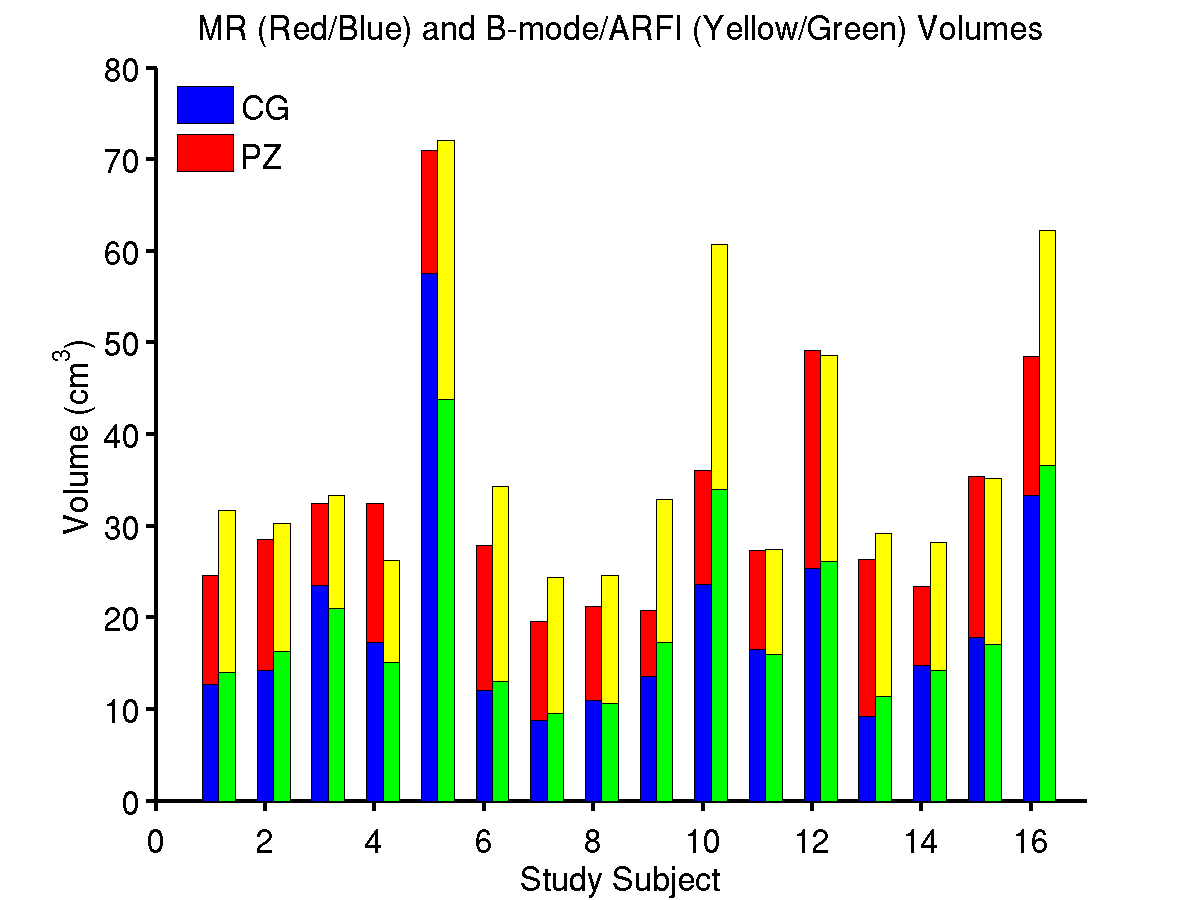
\includegraphics[width=0.3\linewidth]{figs/mr_arfi_volumes} &
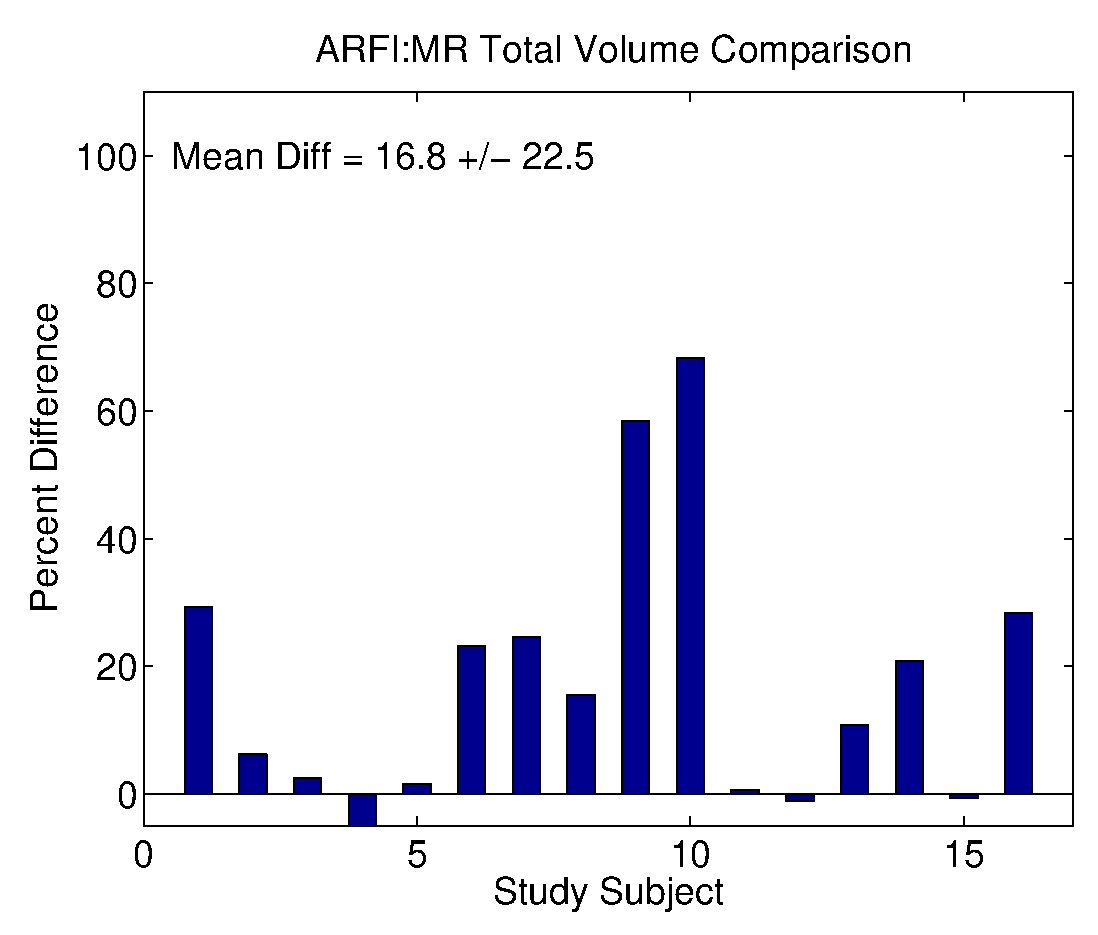
\includegraphics[width=0.3\linewidth]{figs/mr_arfi_volume_diff} &
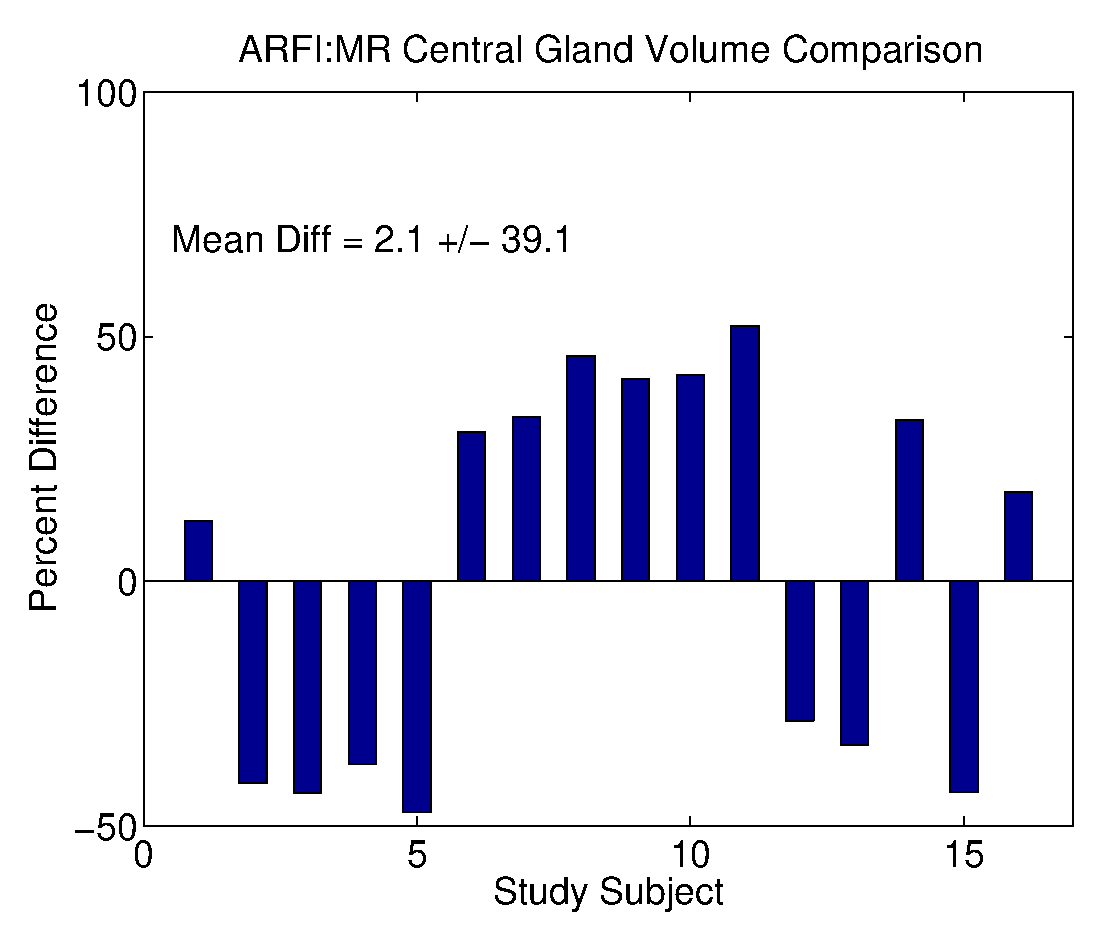
\includegraphics[width=0.3\linewidth]{figs/mr_arfi_central_diff} \\
(a) Central:Peripheral Volume & (b) Total Volume Difference & (c) Central Volume Difference\\
\end{tabular}
\caption{Comparison of MR and ARFI zonal anatomy volume estimates from
    manually-segmented images.  Total prostate volumes ranged from 19.6--71.0
    cm$^3$ based on MR image models (a), with ARFI image models overestimating
    total prostate volume by 36.7 $\pm$ 27.9\% (b).  ARFI image estimation of
    the central zone volume relative to the MR central gland volume varied by
    2.1 $\pm$ 39.0\% (c).  Table~\ref{tab:mr_arfi_volumes} contains the
    individual volume estimates for the entire prostate and the central
    glands.}
\label{fig:mr_arfi_volumes} 
\end{figure}


Weights and axis measurements from the gross pathology processing of the
excised prostates were collected (Table~\ref{tab:path_data}), and using the
axis measurements (lateral-to-lateral, anterior-to-posterior, and
apex-to-base), the prostate volume was approximated as a tri-axial ellipsoid,
and its volume was estimated (\ref{eqn:ellipsoid_volume}).  Prostate weights
were moderately correlated with estimated pathology ellipsoidal prostate
volumes (Figure~\ref{fig:mr_arfi_weight}(a), R$^2$ = 0.68).  There was moderate
correlation between the prostate weight and the image-reconstructed prostate
volumes (Figure~\ref{fig:mr_arfi_weight}(b), R$^2$ = 0.44 (MR) and 0.18
(ARFI)), though there was weaker correlation with the ellipsoidal approximation
of the measurement prostate volume and the image-reconstructed volumes
(Figure~\ref{fig:mr_arfi_weight}(c), R$^2$ = 0.08 (MR) and 0.00 (ARFI)).  

\begin{figure}[htb!]
\centering
\begin{tabular}{lll}
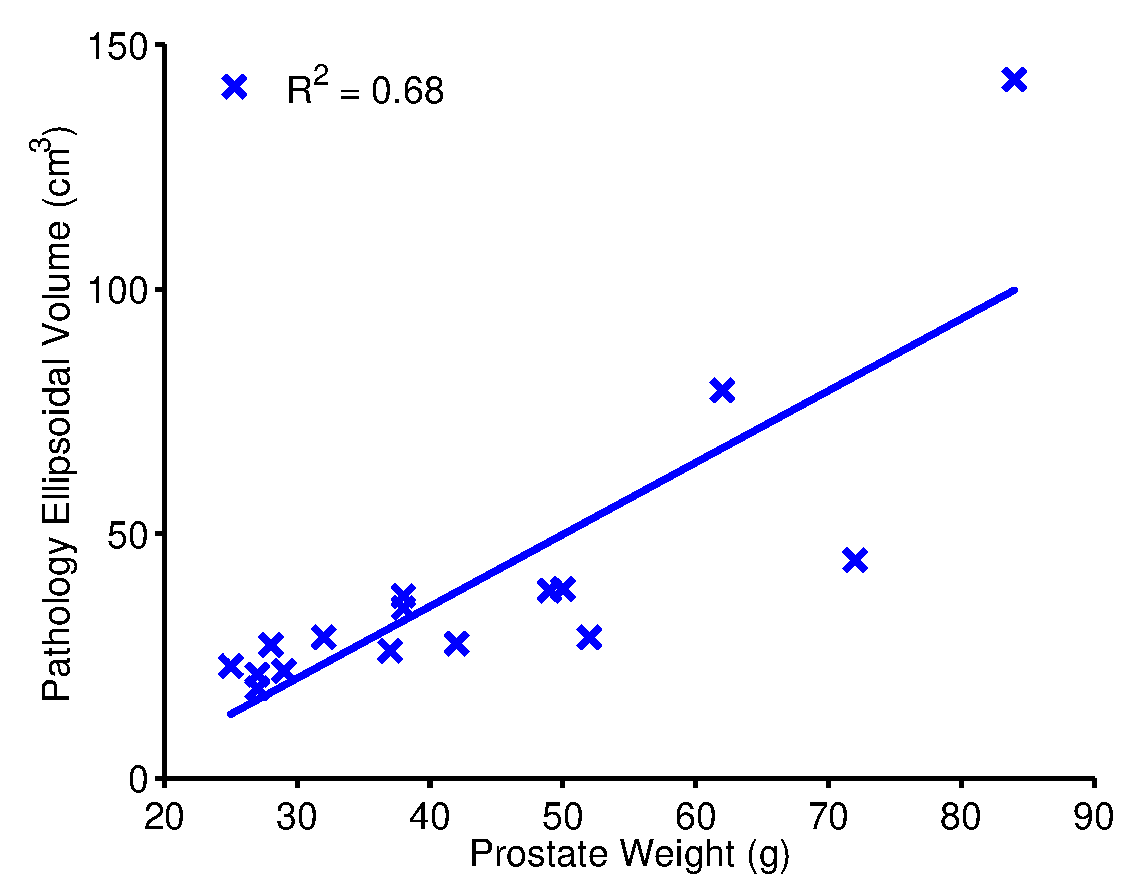
\includegraphics[width=0.3\linewidth]{figs/corr_path_vol_weight_vol} &
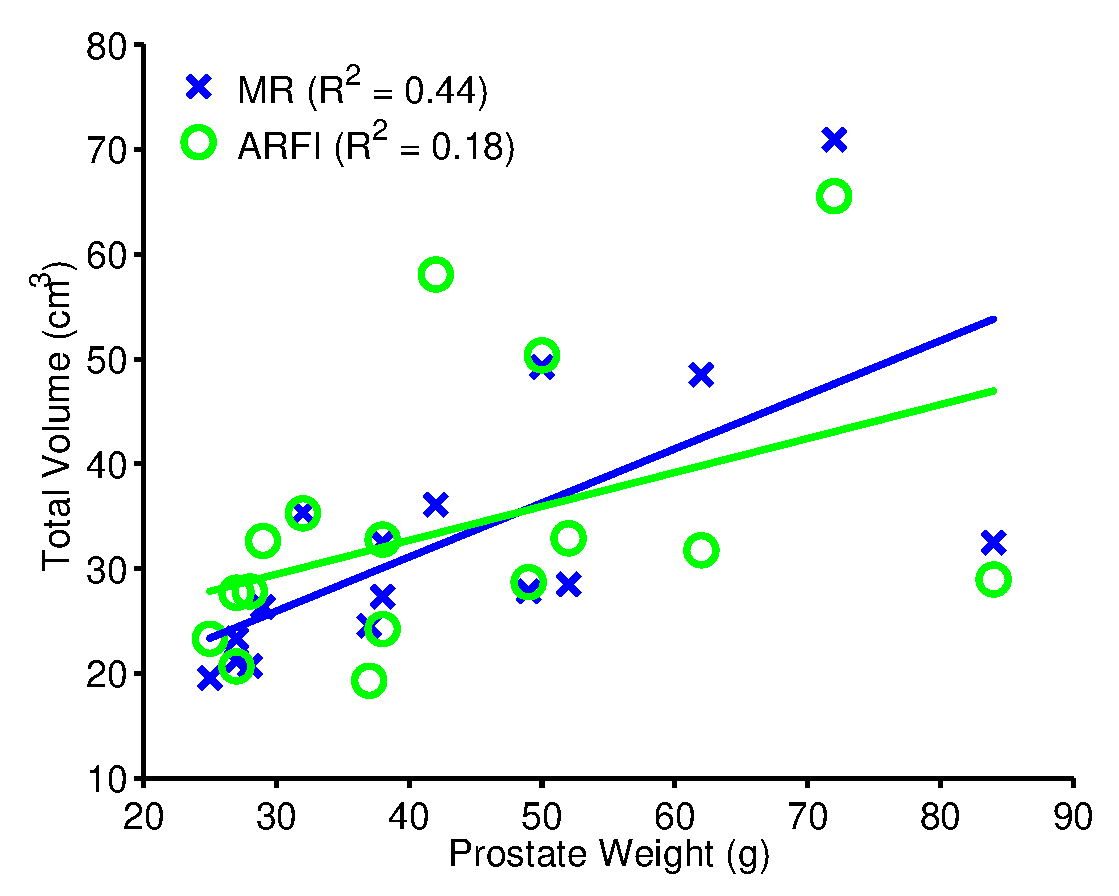
\includegraphics[width=0.3\linewidth]{figs/corr_weight_vol} &
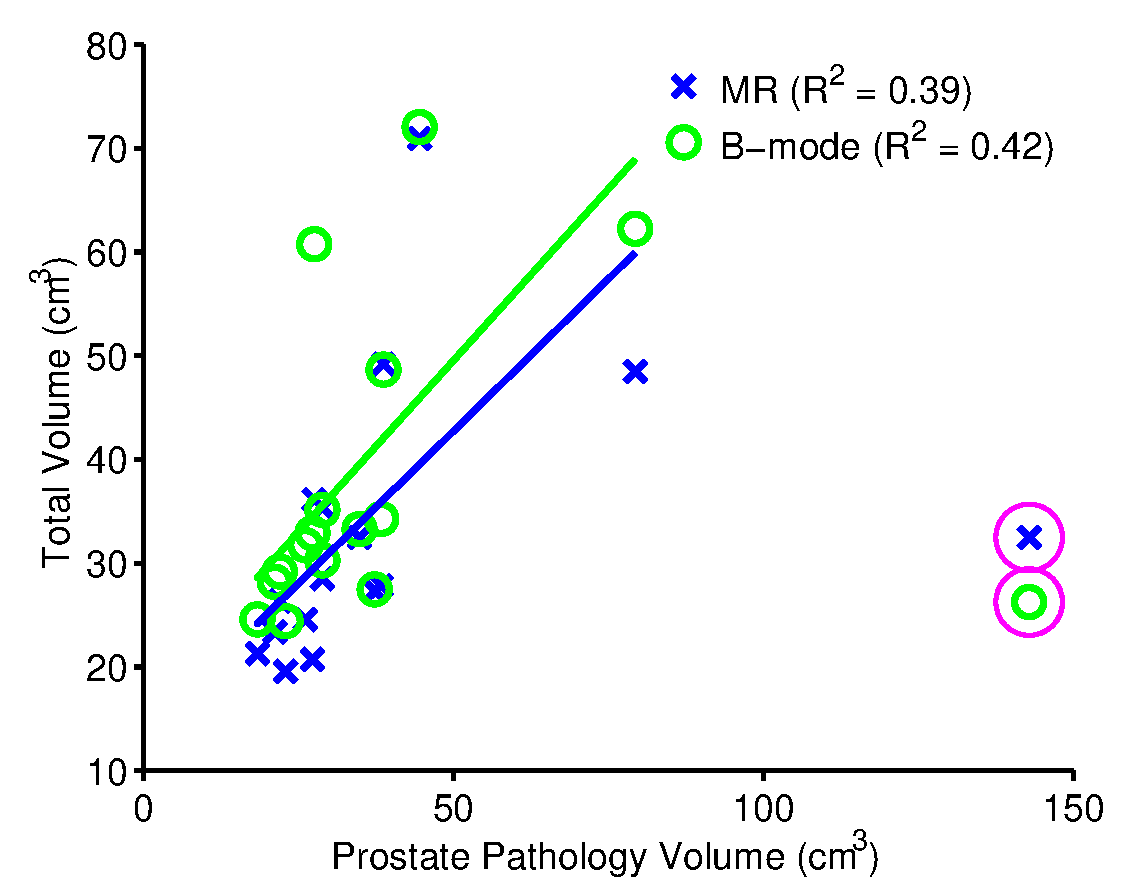
\includegraphics[width=0.3\linewidth]{figs/corr_pathVol_vol} \\
(a) Path Weight : Path Volume & (b) Image Volume : Prostate Weight & (c) Image Volume : Path Volume \\
\end{tabular}
%\begin{tabular}{ll}
%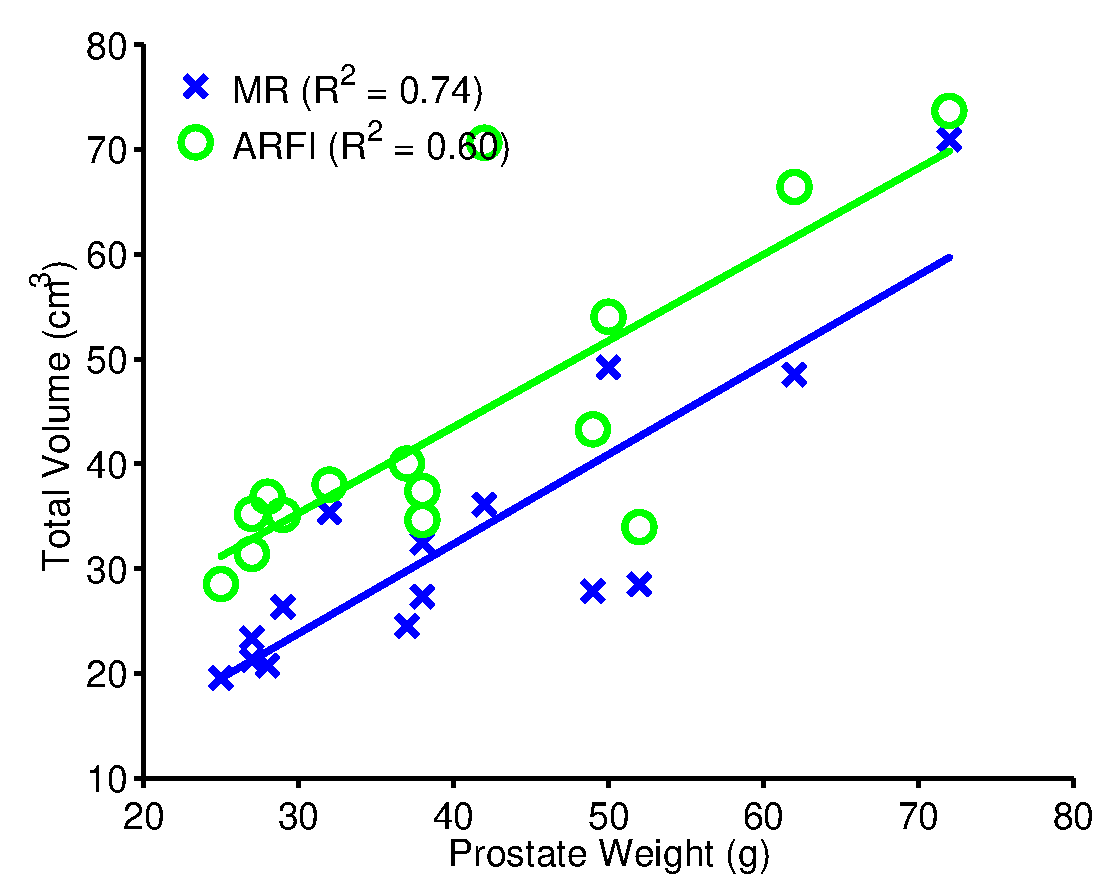
\includegraphics[width=0.3\linewidth]{figs/corr_weight_vol_no4} &
%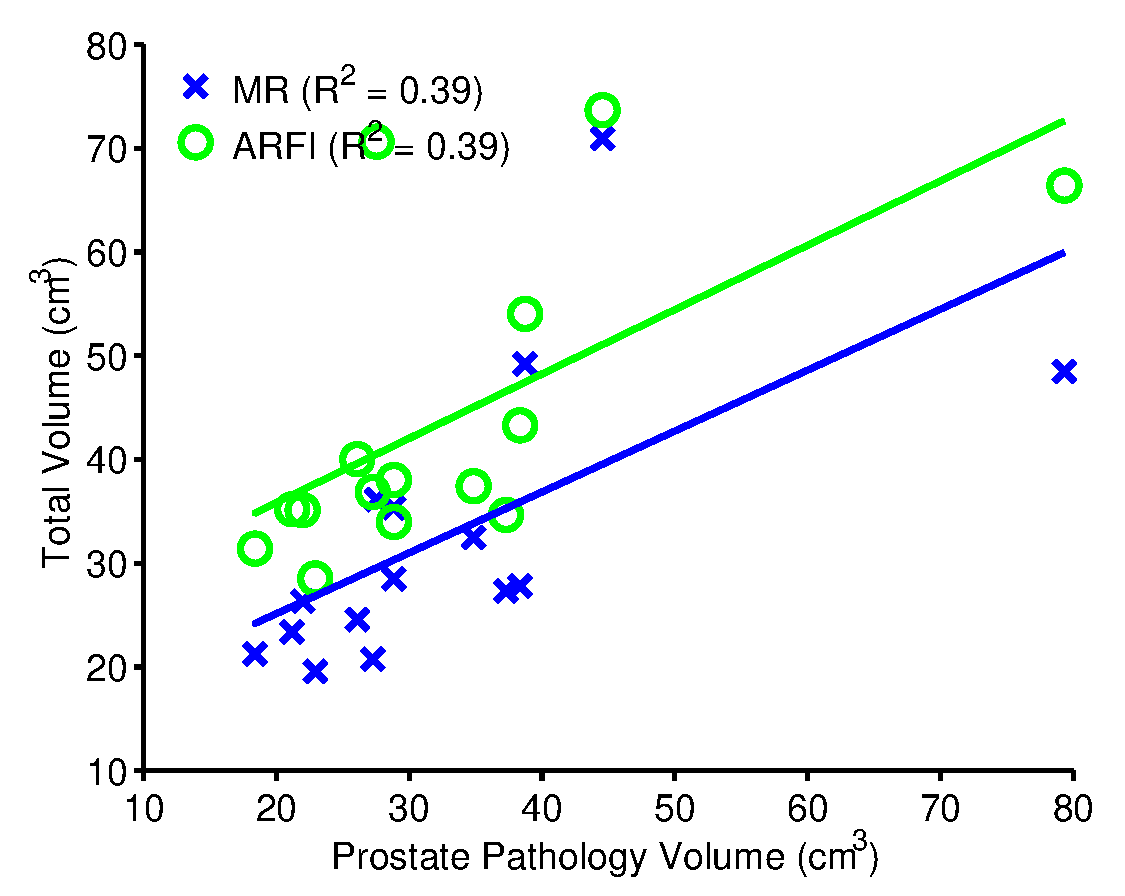
\includegraphics[width=0.3\linewidth]{figs/corr_pathVol_vol_no4} \\
%(d) Image Volume : Prostate Weight (-4) & (e) Image Volume : Path Volume (-4) \\
%\end{tabular}
\caption{Tri-axial pathology measurements were used to make an ellipsoidal
    prostate volume approximation based on gross pathology axis measurements,
    which was moderately well-correlated with the excised prostated weights (a,
    R$^2$ = \pathVolWeightRsq).  T2WI MR (blue, X) showed a moderate
    correlation between the reconstructed volumes and prostate weight (R$^2$ =
    \weightMRrsq), while volumes reconstructed from ARFI images (green, O)
    showed weaker correlation (R$^2$ = \weightARFIrsq) (b).  Weaker
    correlations existed between both T2WI MR and ARFI image volumes and
    approximated ellipsoidal prostate pathology volumes (R$^2$ = \pathVolMRrsq
    and \pathVolARFIrsq, respectively) (c).  One study subject had a very large
    prostate ($>$ 80 g) that was not well visualized by both MR and ARFI
    imaging, and it was excluded from all of the linear regression.  This
    outlier was indicated with magenta circles in the plots.}
\label{fig:mr_arfi_weight}
\end{figure}


Measurements of the prostate total and CG dimensions along the three
standard anatomic axes (apex-to-base, lateral-to-lateral, and
anterior-to-posterior) were made (Table~\ref{tab:mr_arfi_axes}), and the
correlation between the imaging axis measurements was analyzed
(Figure~\ref{fig:mr_arfi_path_axes}).  ARFI was most correlated to MR in the
lateral-to-lateral axis in both the total and CG (R$^2$ = 0.57 and
0.32, respectively), with mean overestimates of 13.5 $\pm$ 11.0\% and 11.5 $\pm$
22.5\%, respectively (Table~\ref{tab:mr_arfi_axes_error}).  ARFI had moderate
correlation with the total prostate gland axis in the anterior-to-posterior
dimension (R$^2$ = 0.23), but poor correlation in the CG (R$^2$ =
0.00), with overestimates of 5.7 $\pm$ 20.6 and -8.4 $\pm$ 24.0\%.  ARFI
imaging had weak correlation with MR images in the apex-to-base dimension
(R$^2$ = 0.19, total gland and R$^2$ = 0.09, CG), with differences
of -2.4 $\pm$ 17.0 and 1.2 $\pm$ 19.8\%, respectively.

\begin{figure}
\centering
\begin{tabular}{ccc}
%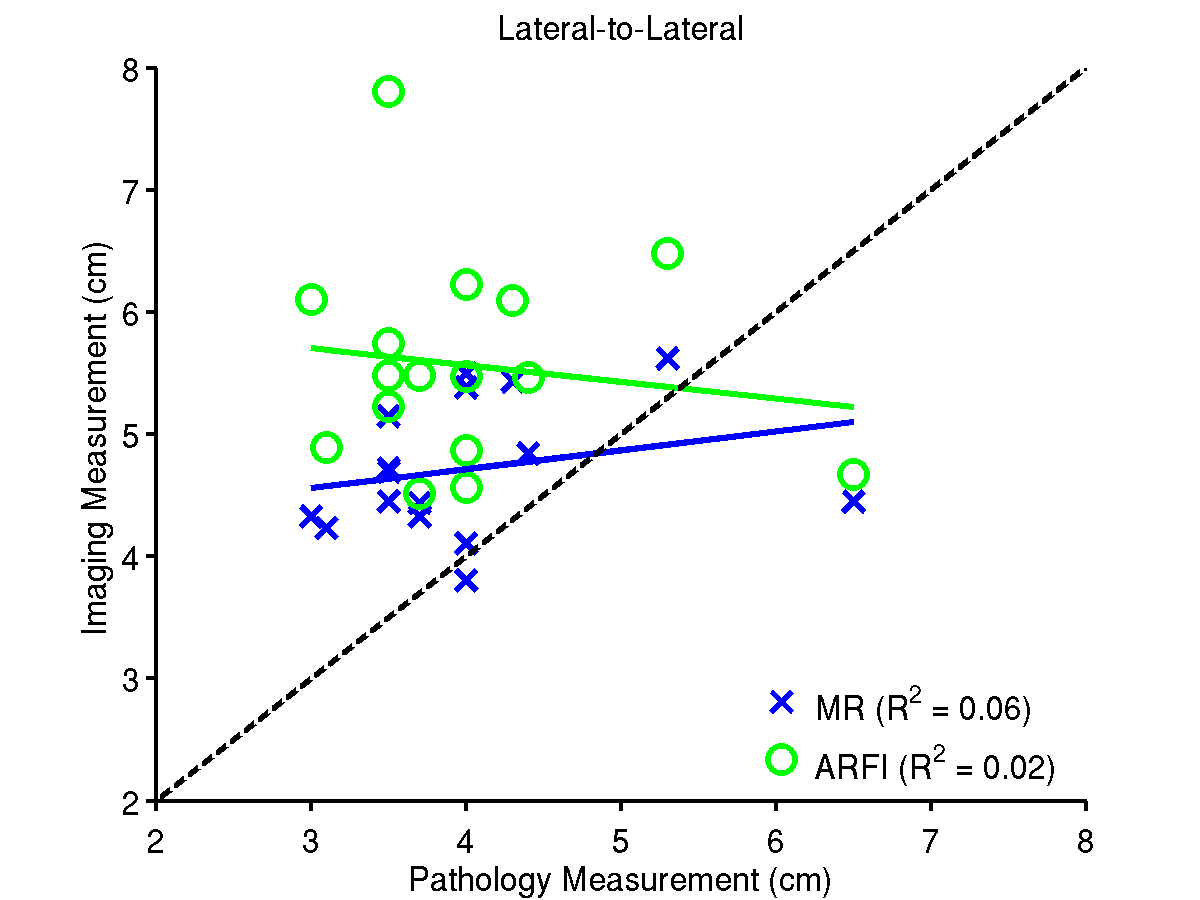
\includegraphics[width=0.3\linewidth]{figs/Lateral-to-Lateral} &
%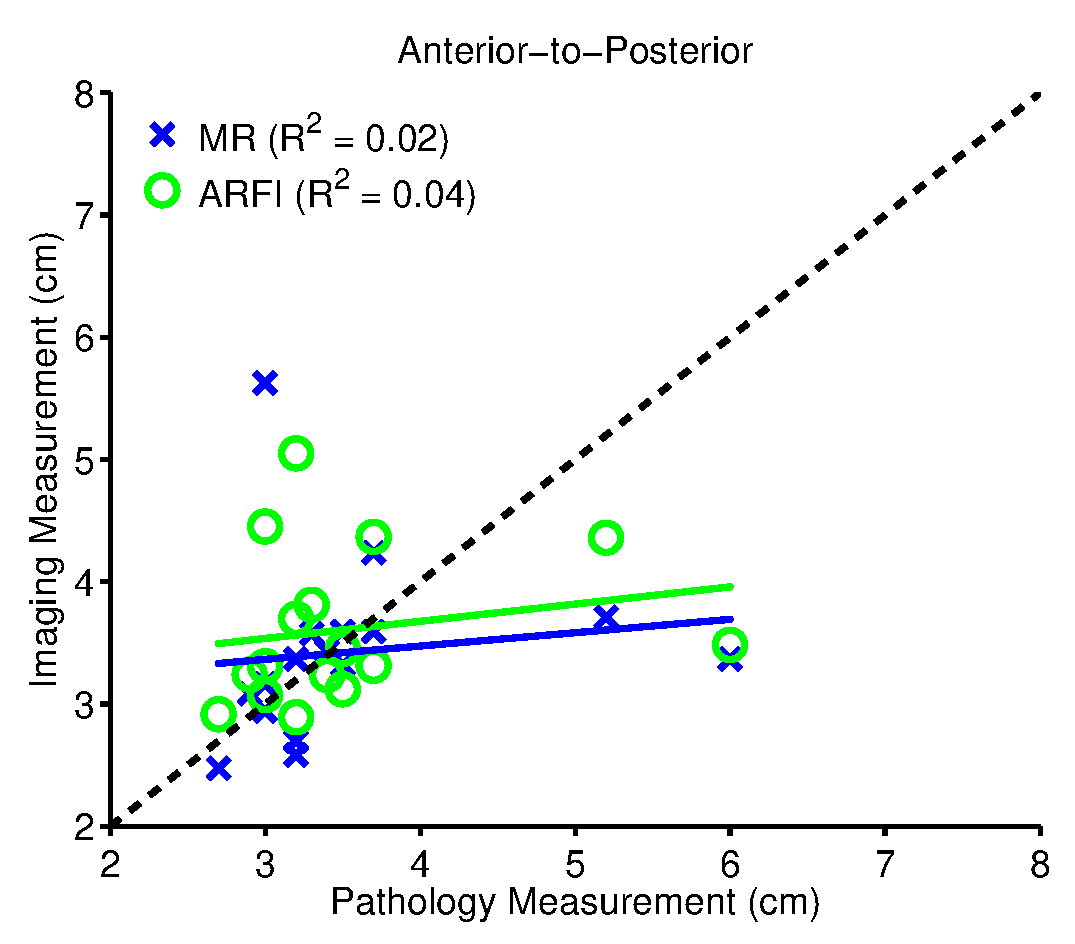
\includegraphics[width=0.3\linewidth]{figs/Anterior-to-Posterior} &
%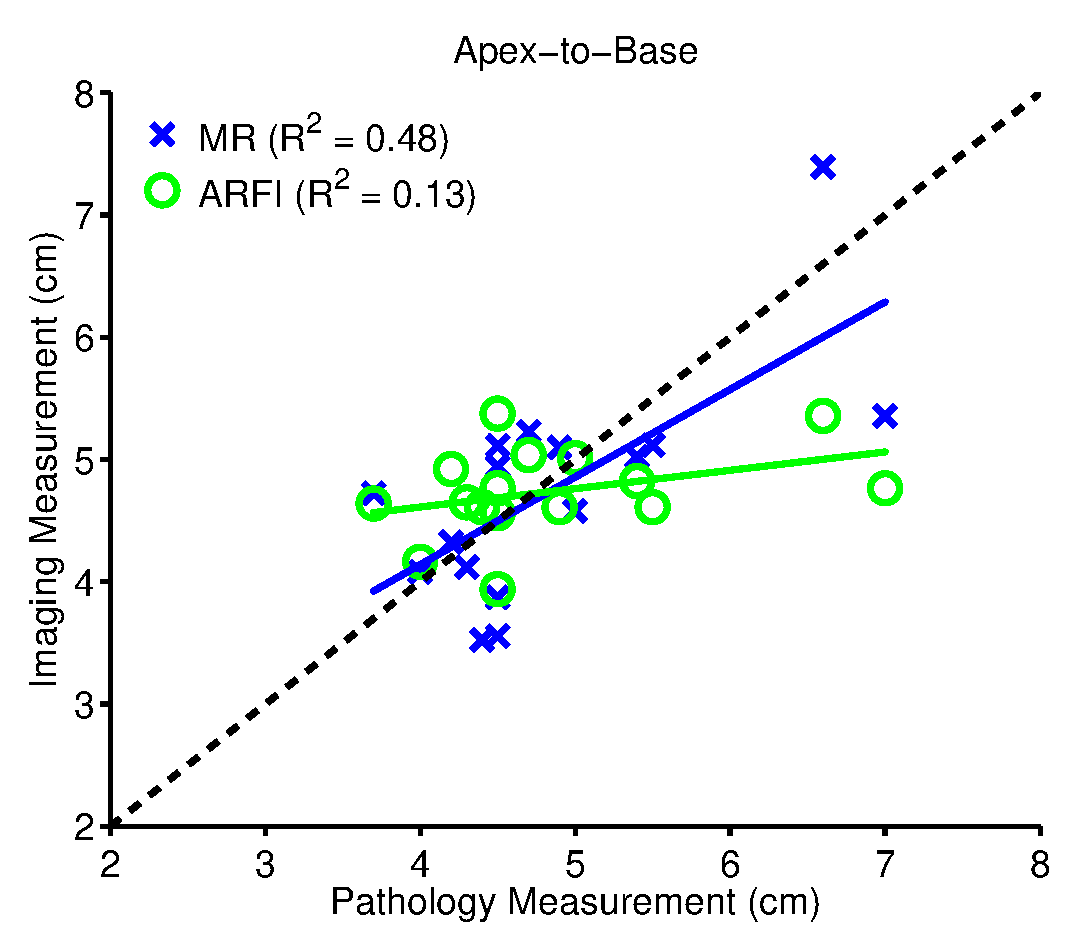
\includegraphics[width=0.3\linewidth]{figs/Apex-to-Base} \\
%(a) & (b) & (c) \\
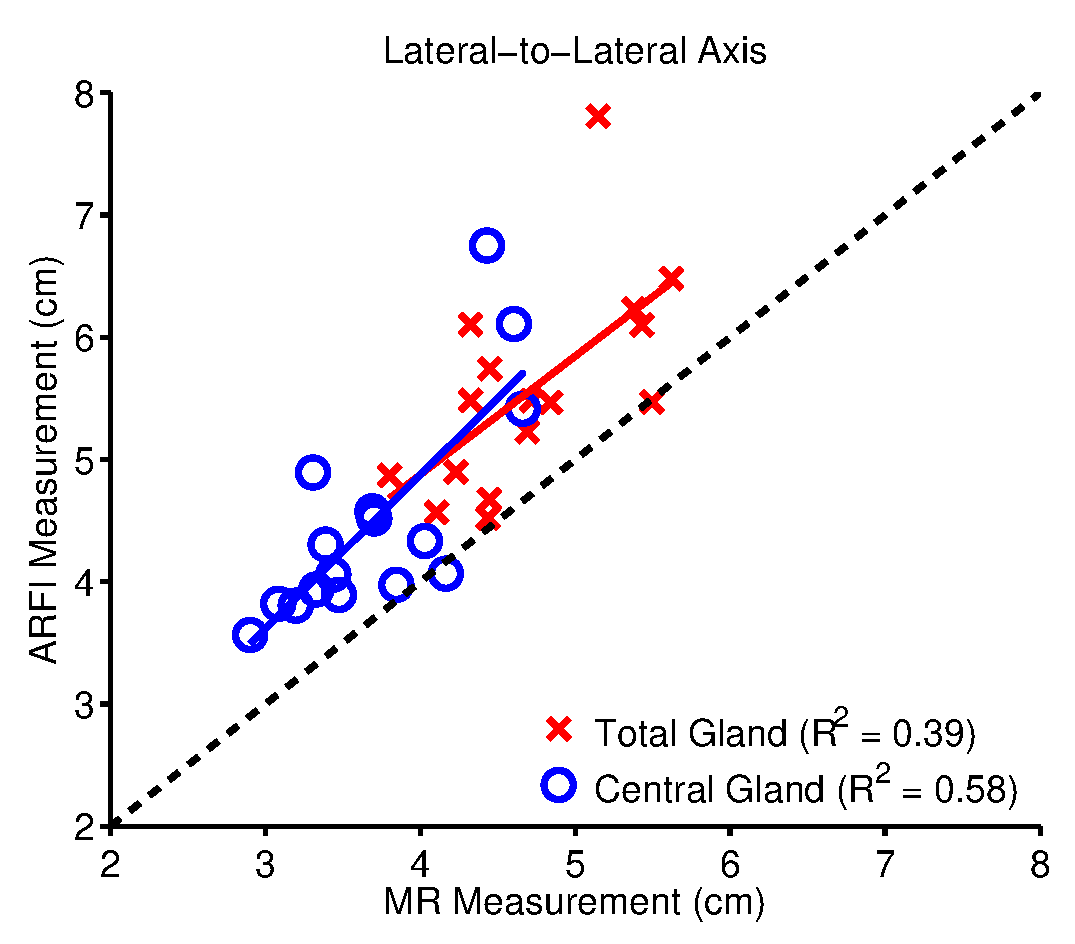
\includegraphics[width=0.3\linewidth]{figs/Imaging_Lateral-to-Lateral} &
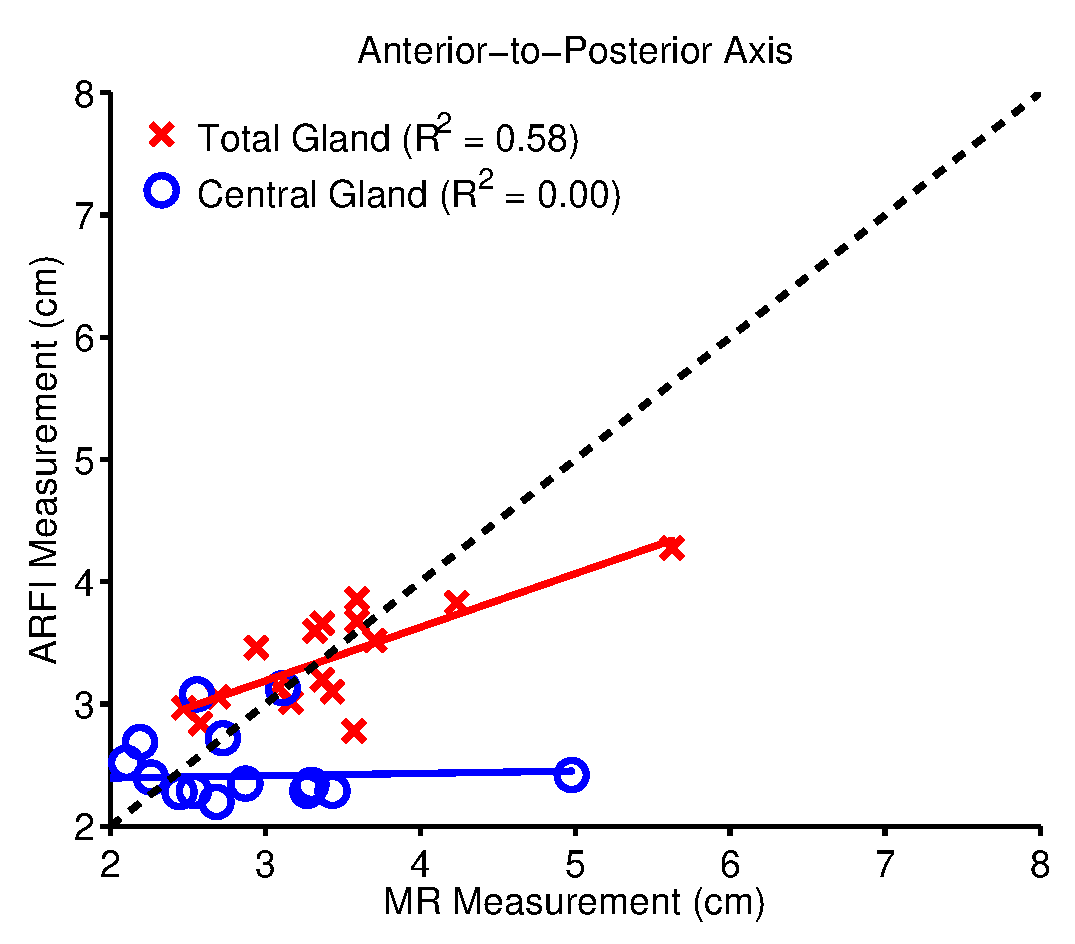
\includegraphics[width=0.3\linewidth]{figs/Imaging_Anterior-to-Posterior} &
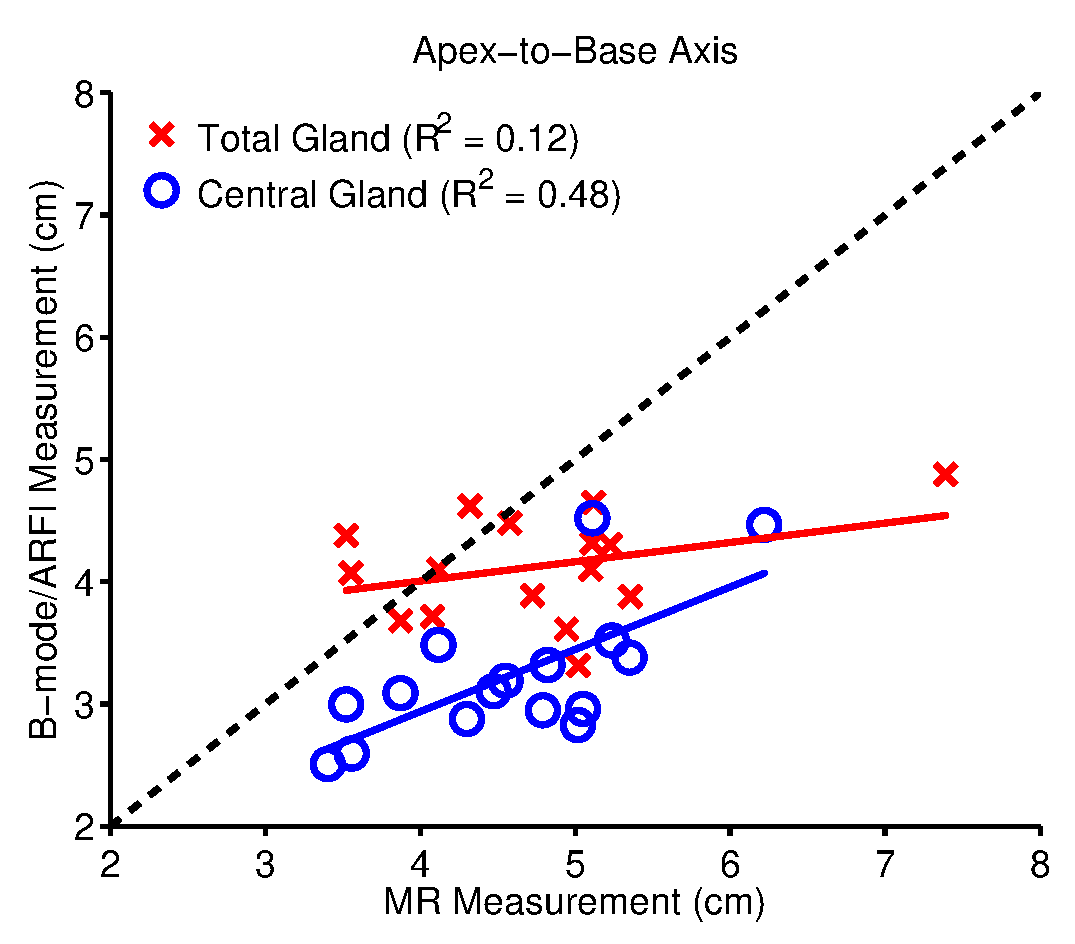
\includegraphics[width=0.3\linewidth]{figs/Imaging_Apex-to-Base} \\
(a) & (b) & (c) \\
%(d) & (e) & (f) \\
\end{tabular}
\caption{Measurements of the prostate dimensions along the three standard
    anatomic axes: lateral-to-lateral (a), anterior-to-posterior (b) and
    apex-to-base (c).  The correlation between the MR and B-mode/ARFI imaging
    axis measurements was performed in each orientation for the total gland
    (red crosses) and central gland (blue circles).  \textbf{B-mode images were
        used for total gland measurements, and ARFI images were for central
        gland measurements.} The black dashed-line represents the projection of
    perfectly-correlated measurements between imaging and pathology.  The
    over-/under-estimation of each imaging modality relative to gross pathology
    and each other is summarized in Table~\ref{tab:mr_arfi_axes_error}.} 
\label{fig:mr_arfi_path_axes}
\end{figure}


\begin{table}[h!]
\centering
\caption{Difference in ARFI imaging axis measurements relative to MR T2WI measurements.}
\begin{tabular}{|l|l|l|} \hline
 & {\bf ARFI:MR} & {\bf ARFI:MR} \\
 & {\bf Total Gland (\%)} & {\bf Central Gland (\%)} \\ \hline
{\bf Lateral-to-Lateral} & 8.1 $\pm$ 18.4 & 0.06 $\pm$ 17.2 \\
{\bf Anterior-to-Posterior} & 17.0 $\pm$ 12.1 & 14.8 $\pm$ 23.1 \\
{\bf Apex-to-Base} & 0.58 $\pm$ 12.9 & -10.8 $\pm$ 22.3 \\
\hline
\end{tabular}
\label{tab:mr_arfi_axes_error}
\end{table}


%\begin{figure}
\centering
\begin{tabular}{ccc}
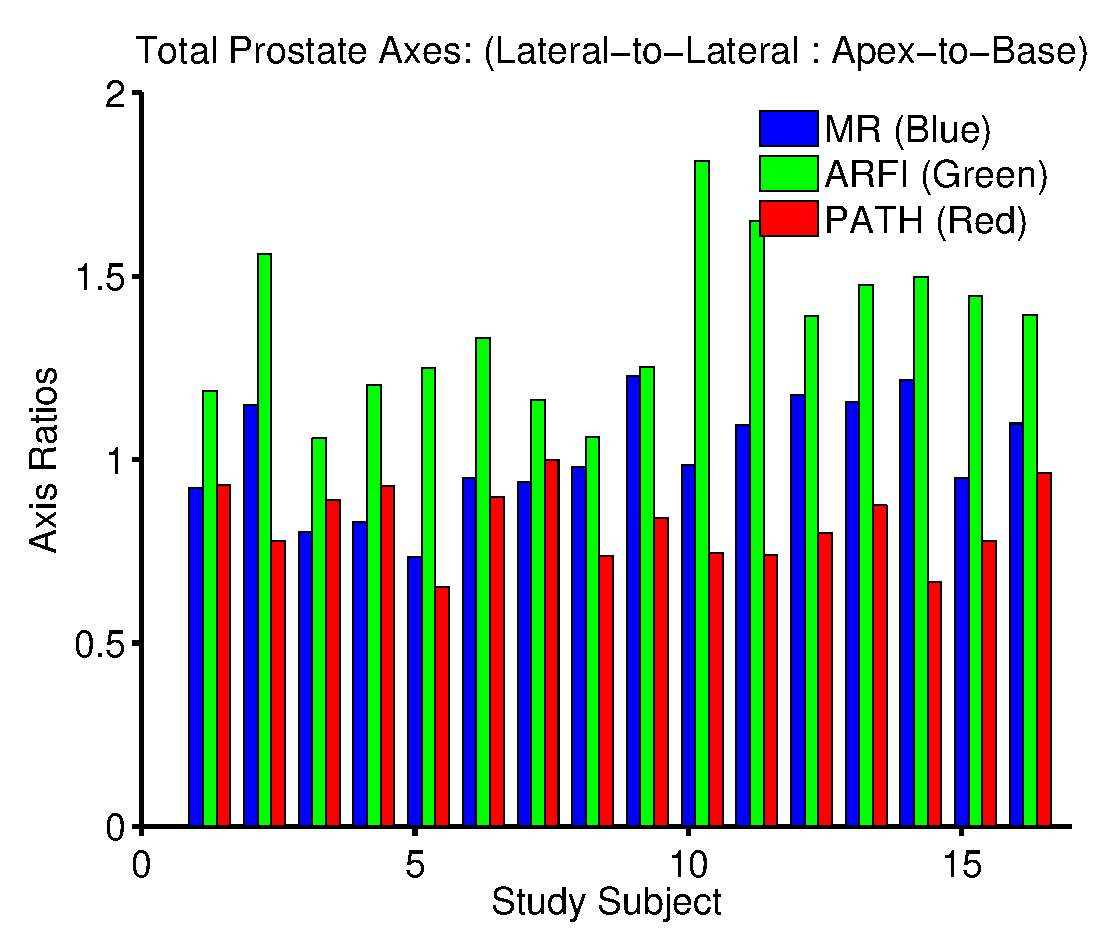
\includegraphics[width=0.3\linewidth]{figs/mr_arfi_total_axes1} &
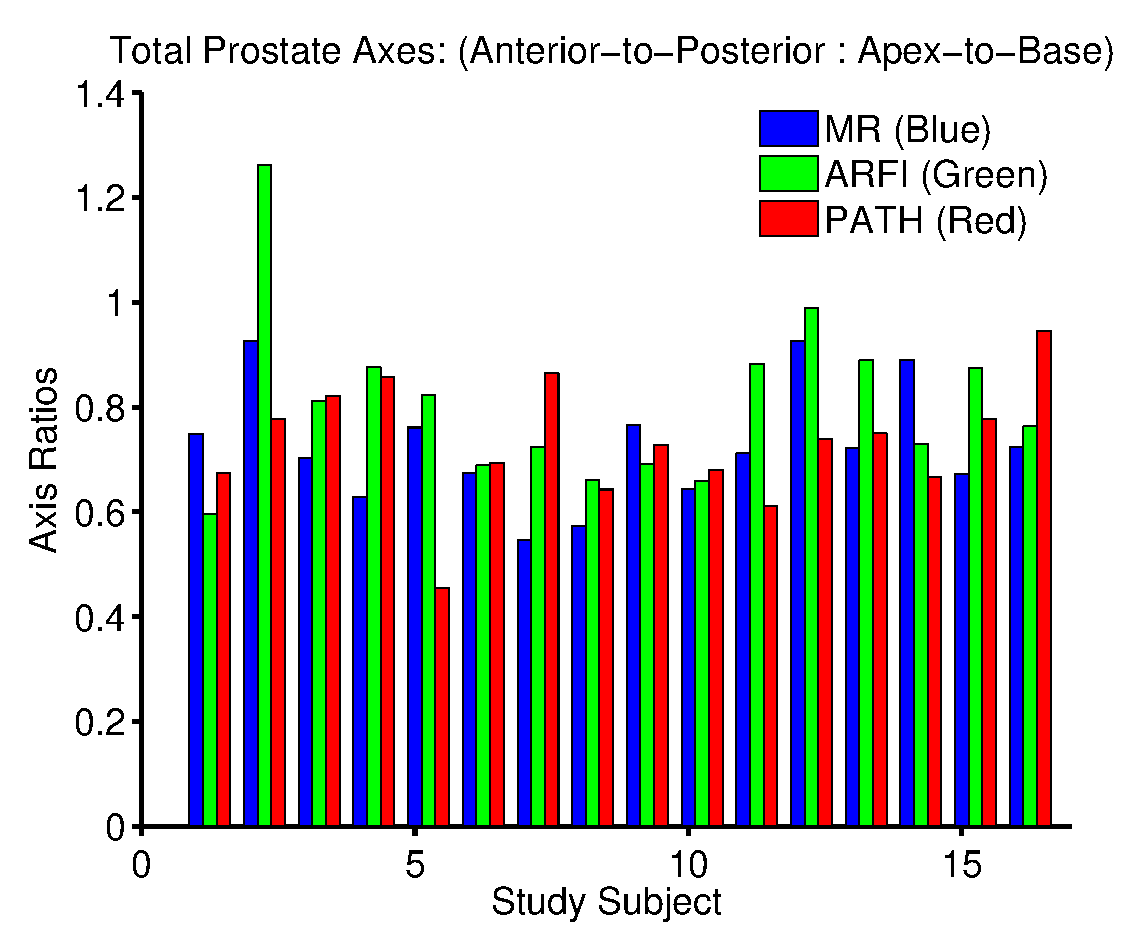
\includegraphics[width=0.3\linewidth]{figs/mr_arfi_total_axes2} &
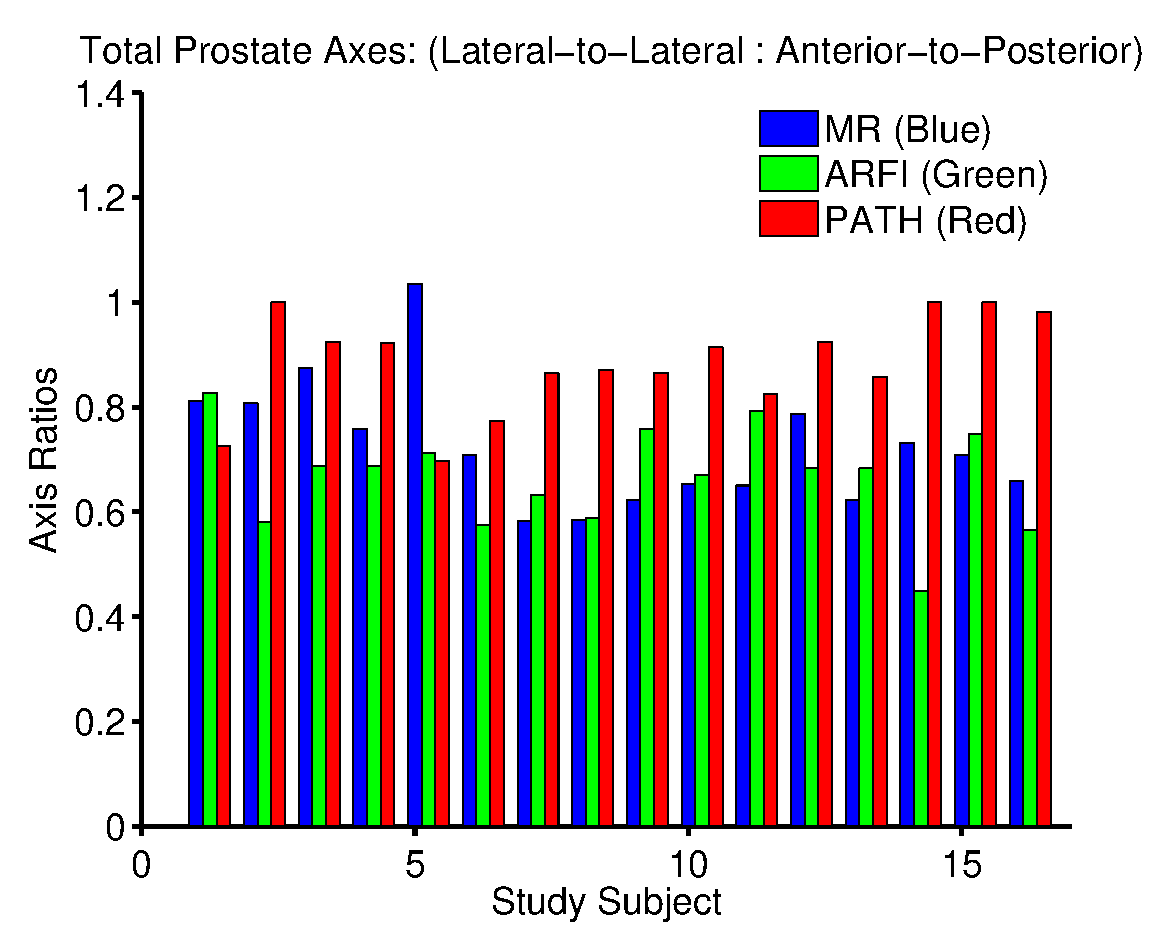
\includegraphics[width=0.3\linewidth]{figs/mr_arfi_total_axes3} \\
(a) & (b) & (c) \\
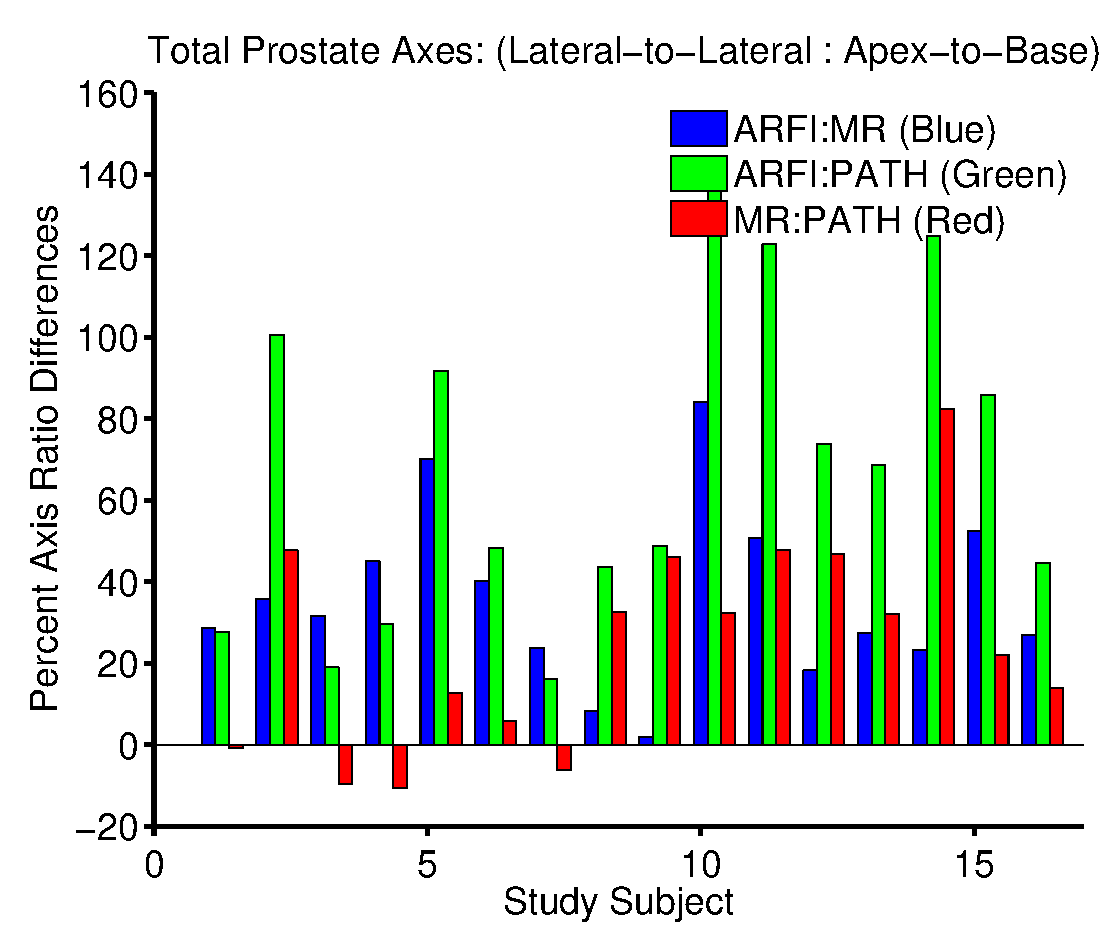
\includegraphics[width=0.3\linewidth]{figs/mr_arfi_total_over_under1} &
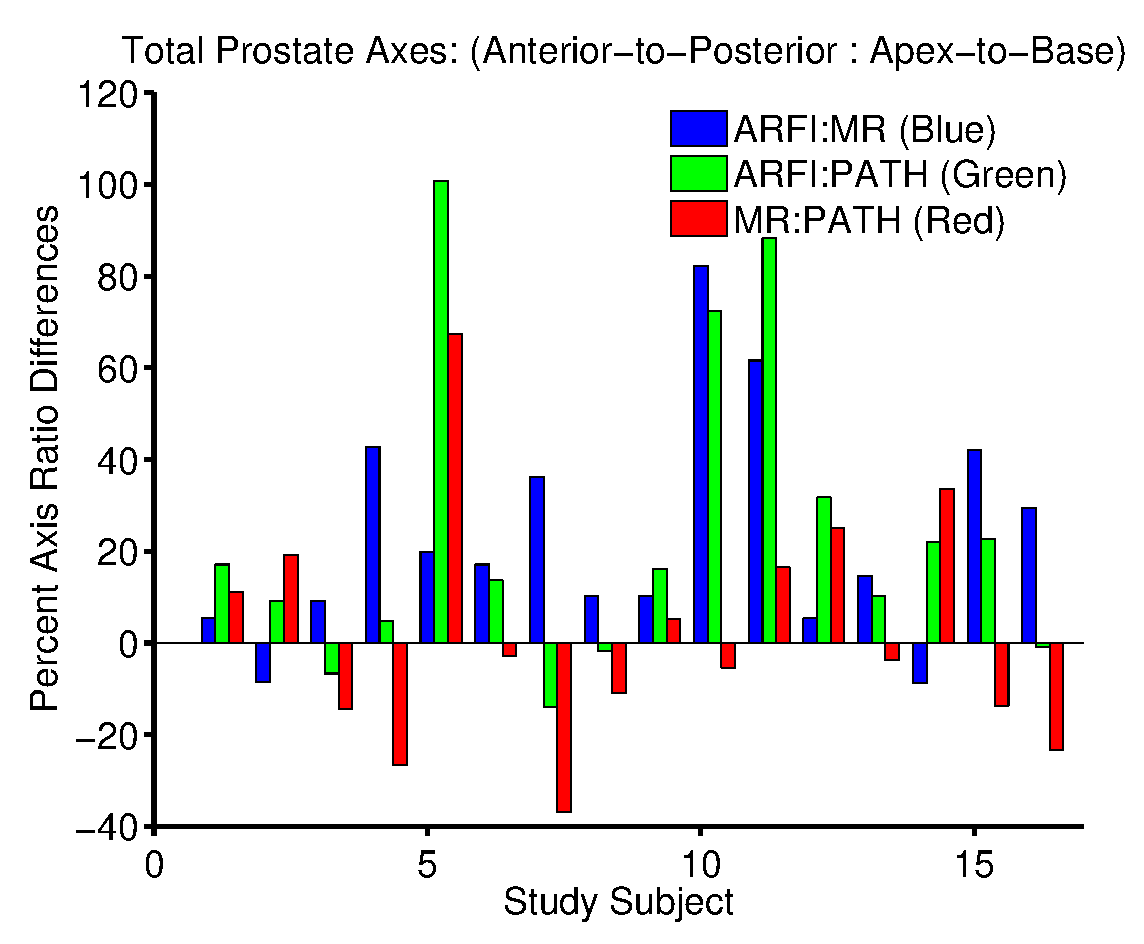
\includegraphics[width=0.3\linewidth]{figs/mr_arfi_total_over_under2} &
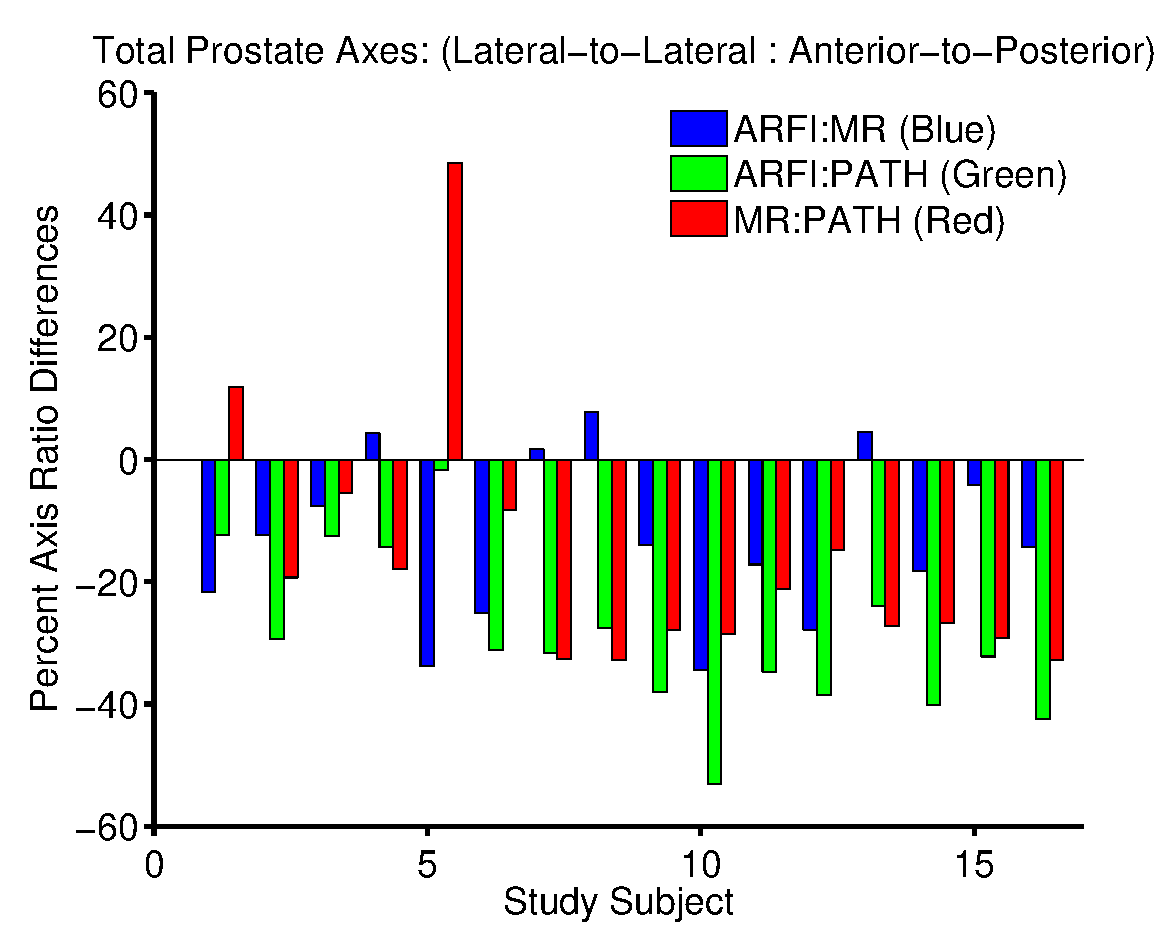
\includegraphics[width=0.3\linewidth]{figs/mr_arfi_total_over_under3} \\
(d) & (e) & (f) \\
\end{tabular}
\caption{Comparison of the ratios of the three anatomic axis measurement ratios
    for T2WI MR (top row, blue), ARFI imaging (top row, green) and gross
    pathology (top row, red).  The over/underestimation of the axis ratios
    between ARFI imaging : T2WI MR : Pathology are shown in the bottom row
    (d-f), with mean ratio differences compiled in
    Table~\ref{tab:axis_ratio_over_under}.}
\label{fig:mr_arfi_total_axes} 
\end{figure}


%\begin{figure}
\centering
\begin{tabular}{ccc}
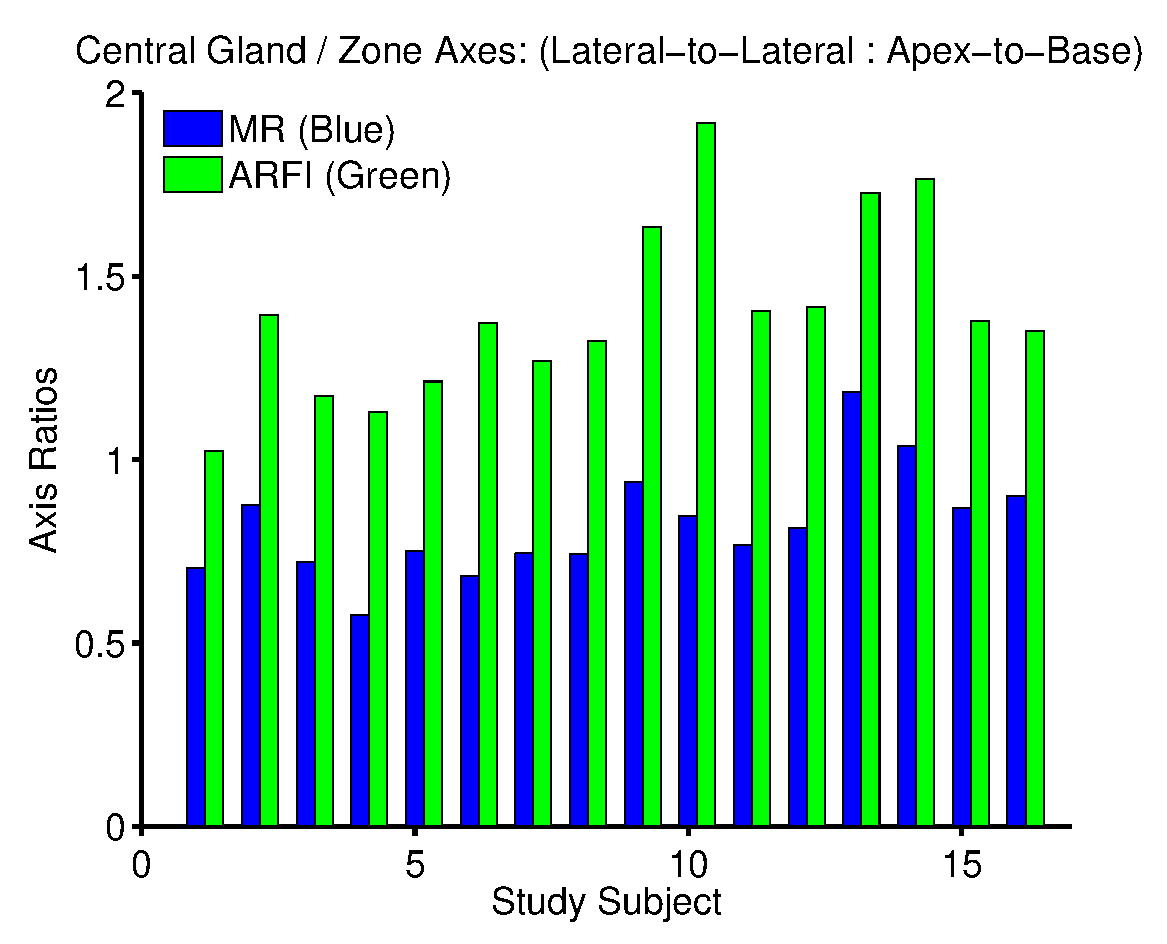
\includegraphics[width=0.3\linewidth]{figs/mr_arfi_central_axes1} &
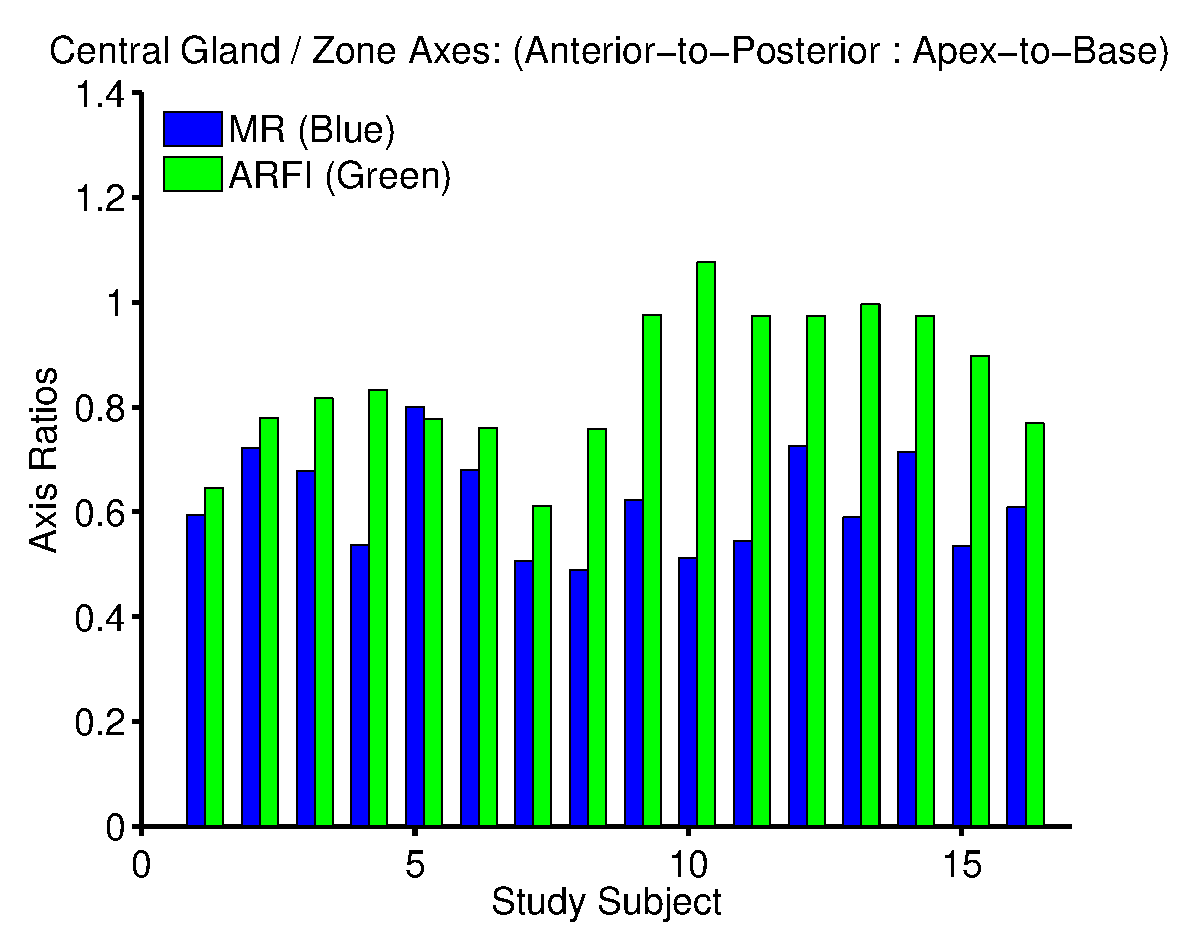
\includegraphics[width=0.3\linewidth]{figs/mr_arfi_central_axes2} &
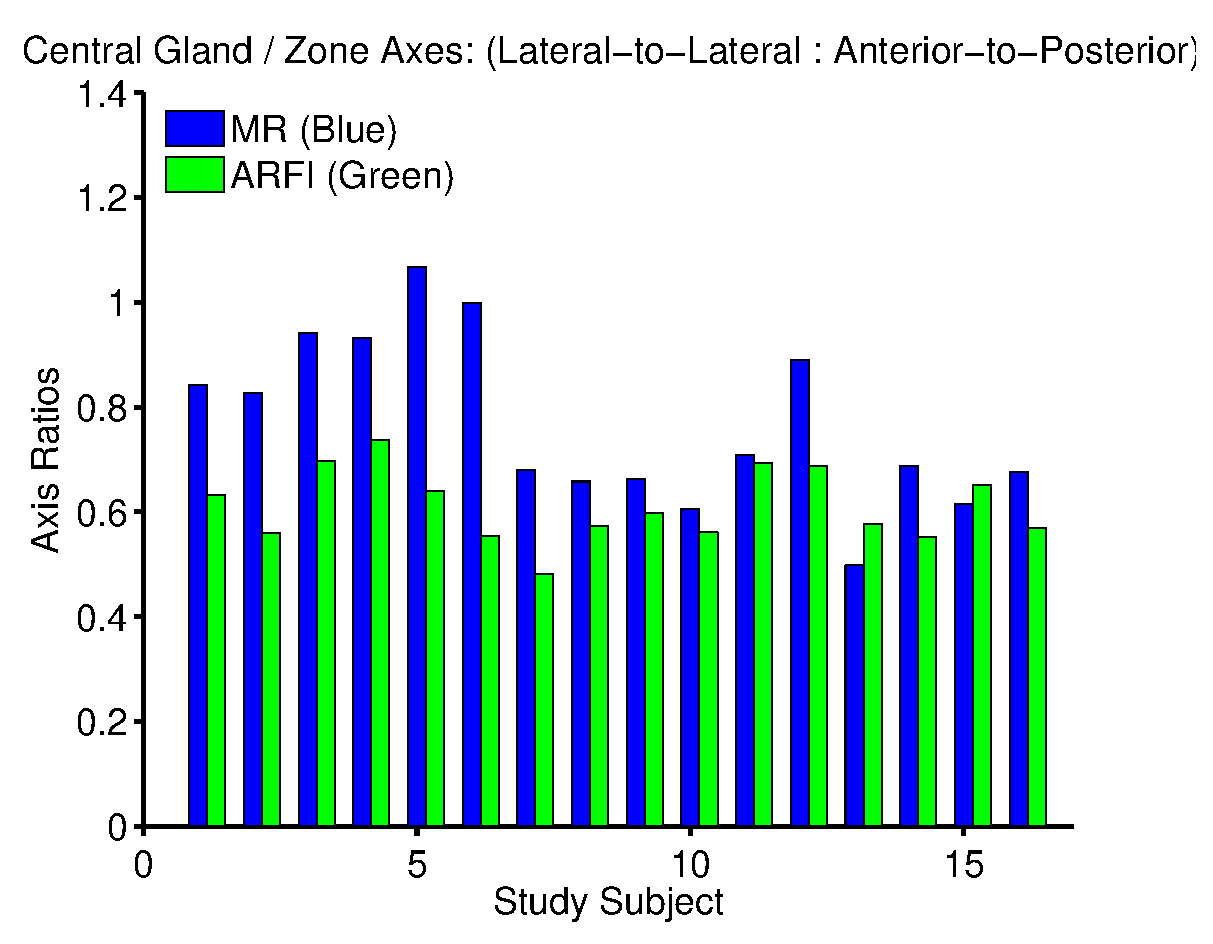
\includegraphics[width=0.3\linewidth]{figs/mr_arfi_central_axes3} \\
(a) & (b) & (c) \\
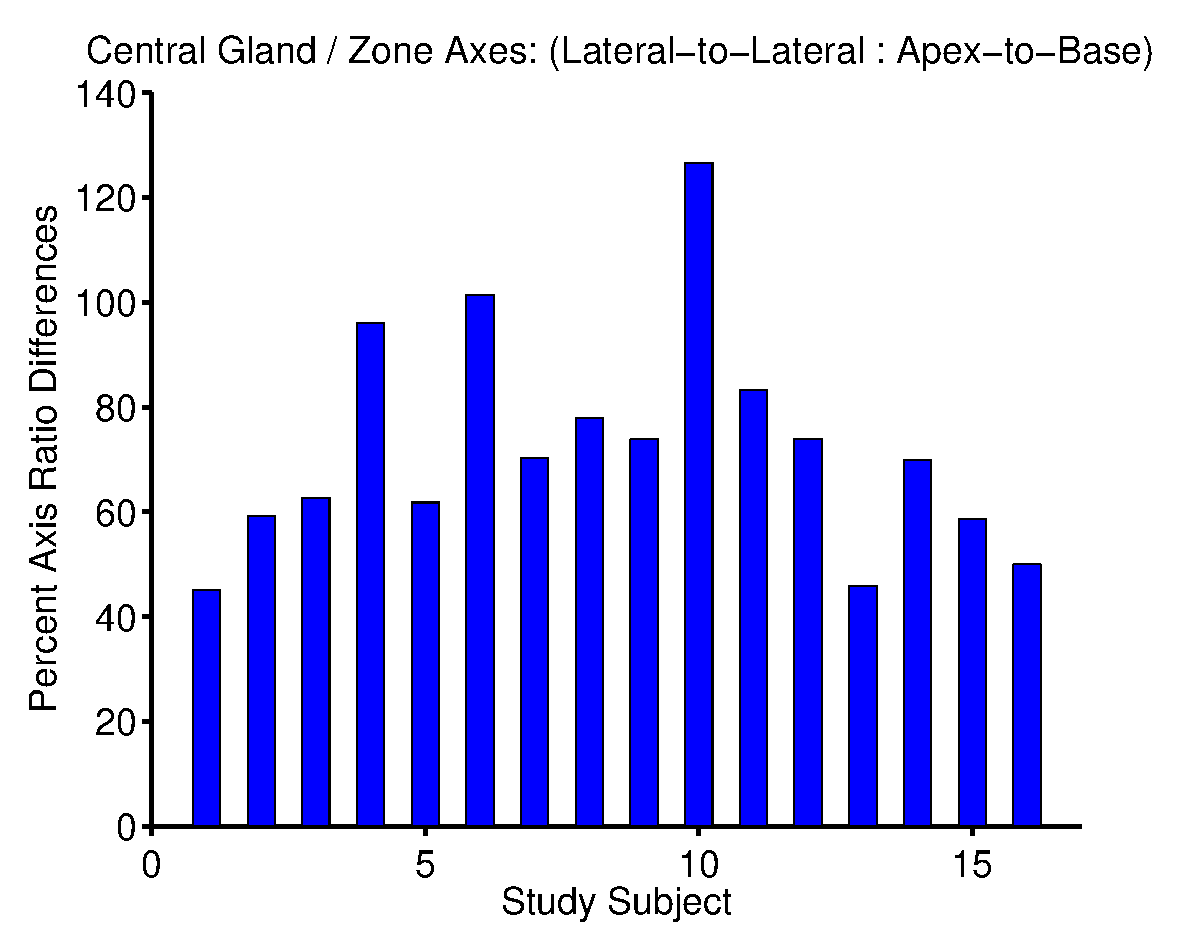
\includegraphics[width=0.3\linewidth]{figs/mr_arfi_central_over_under1.eps} &
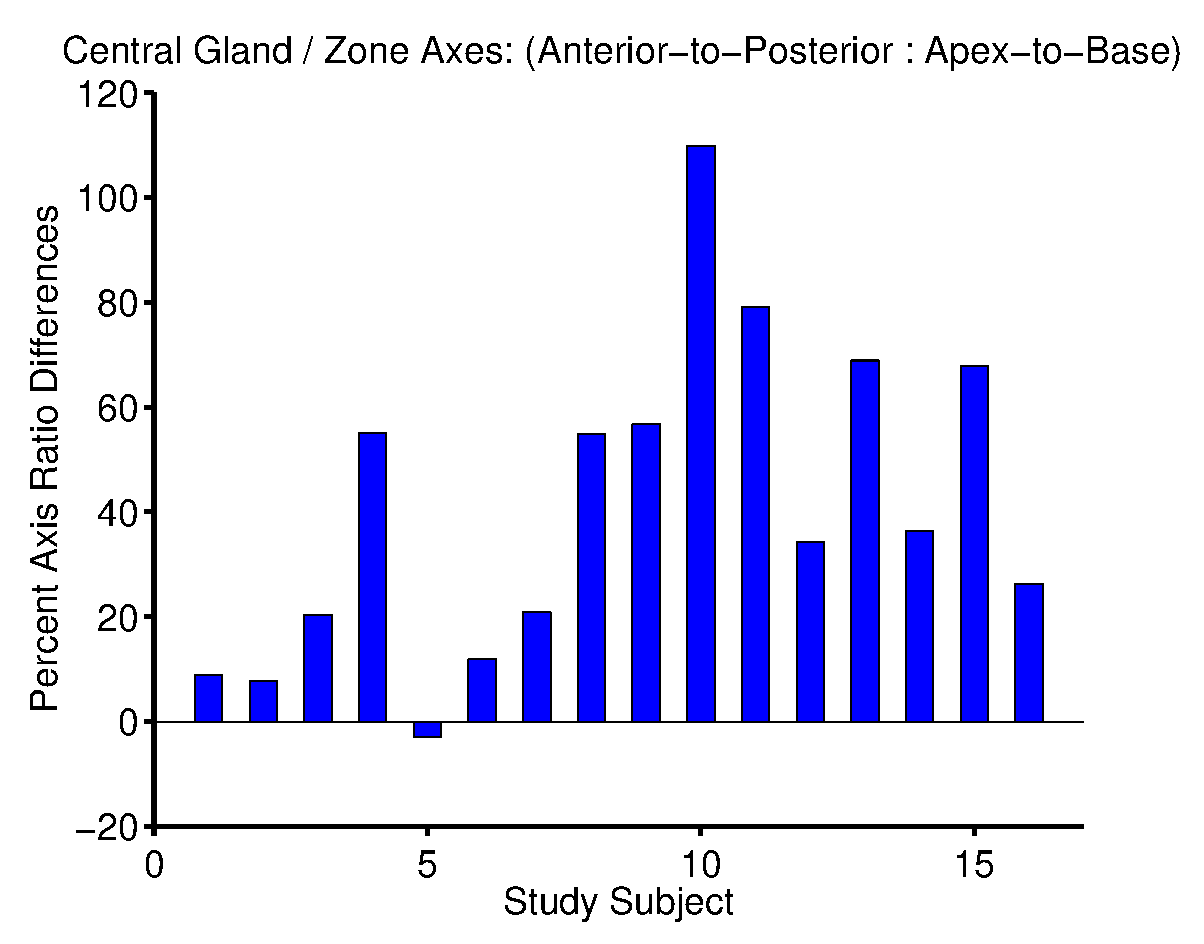
\includegraphics[width=0.3\linewidth]{figs/mr_arfi_central_over_under2.eps} &
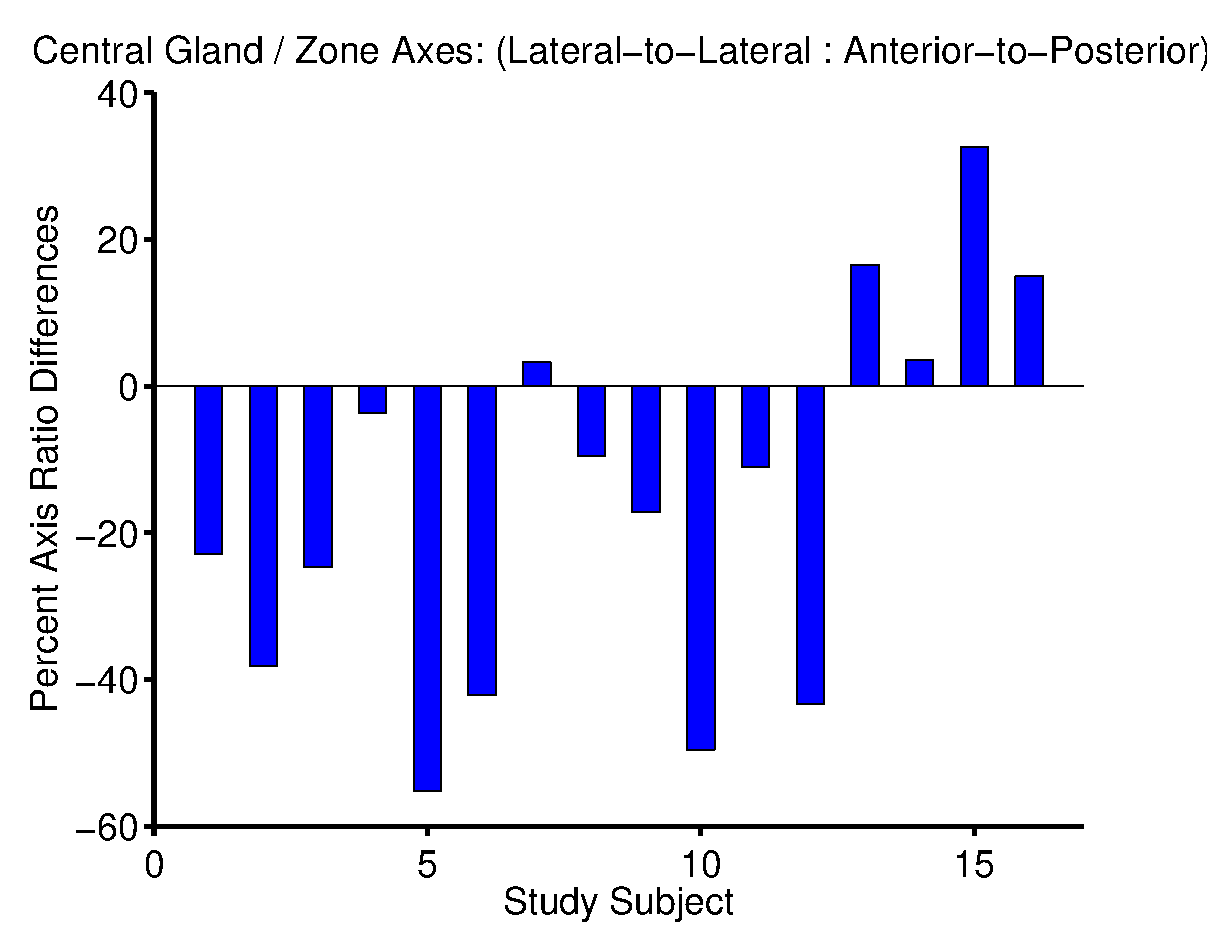
\includegraphics[width=0.3\linewidth]{figs/mr_arfi_central_over_under3.eps} \\
(a) & (b) & (c) \\
\end{tabular}
\caption{Comparison of the ratios of the three anatomic axis measurement ratios
    for T2WI MR (top row, blue) and ARFI imaging (top row, green).  The
    over/underestimation of the axis ratios between ARFI imaging and T2WI MR
    are shown in the bottom row (d-f), with mean ratio differences compiled in
    Table~\ref{tab:axis_ratio_over_under}.}
\label{fig:mr_arfi_central_axes} 
\end{figure}


%\begin{table}
\centering
\caption{Mean axis ratio differences between ARFI imaging, T2WI MR and
    pathology for the total prostate volume and central gland / zone for the
    imaging modalities.  The three axis ratios analyzed were:
    lateral-to-lateral : apex-to-base (LL:AB), anterior-to-posterio :
    apex-to-base (AP:AB), and lateral-to-lateral : anterior-to-posterior
    (LL:AP).}
\begin{tabular}{|l|l|l|l|l|} \hline
{\bf Image Modality} & {\bf Comparative Measure} & {\bf Total / Central} & {\bf Axes} & {\bf Axis Ratio Difference (\%)} \\ \hline
ARFI & MR & Total & LL:AB & 13.9 $\pm$ 22.9 \\ 
ARFI & PATH & Total & LL:AB & 39.3 $\pm$  27.6 \\ 
MR & PATH & Total & LL:AB & 24.7 $\pm$ 26.0 \\ 
ARFI & MR & Total & AP:AB & 5.2 $\pm$ 22.6 \\ 
ARFI & PATH & Total & AP:AB & 5.4 $\pm$  28.3 \\ 
MR & PATH & Total & AP:AB & 2.5 $\pm$ 26.0 \\ 
ARFI & MR & Total & LL:AP & -6.4 $\pm$ 18.3 \\ 
ARFI & PATH & Total & LL:AP & -23.3 $\pm$  17.1 \\ 
MR & PATH & Total & LL:AP & -16.5 $\pm$ 21.1 \\ 
ARFI & MR & Central & LL:AB & 12.0 $\pm$ 22.5 \\ 
ARFI & MR & Central & AP:AB & -6.1 $\pm$ 18.9 \\ 
ARFI & MR & Central & LL:AP & -13.3 $\pm$ 23.7 \\ 

\hline
\end{tabular}
\label{tab:axis_ratio_over_under}
\end{table}



\section{Discussion}\label{sect:discussion}
This study demonstrated that ARFI imaging delineates zonal anatomy of the
prostate well when compared to MR T2WI, with comparable estimates of total and
central gland volume (Figure~\ref{fig:mr_arfi_volumes}).  Establishing accurate
delineation of the prostate's zonal anatomy is important since PCa has a strong
correlations with location in the prostate, specifically in the peripheral
zone, and accurate capsule delineation will facilitate future efforts to
register 3D imaging datasets between ARFI and MR imaging.  

This was the first quantitative comparison between ARFI imaging and a newly
established clinical imaging modality to evaluate the prostate for PCa
detection and characterization, and we have drawn some useful conclusions in
how our zonal anatomy boundaries are determined during image segmentation.
Poor contrast between the PZ and peri-prostatic fat in B-mode images can lead
to an overestimation of lateral boundaries of the prostate in our ultrasound
datasets compared to MR T2WI, leading to an overall overestimation of prostate
total gland volume.  The anterior aspect of the prostate can also be
challenging to delineate, especially in large prostates, where SNR decreases
with increasing depth away from our rectal wall imaging surface and MR images
suffer from gland heterogeneity in this region~\cite{Gupta2013}, though we had
good agreement between ARFI and MR T2W images in the anterior-to-posterior
dimension (Figure~\ref{fig:mr_arfi_path_axes}(b),
Table~\ref{tab:mr_arfi_axes_error}).  Surprisingly, ARFI imaging consistently
underestimated the extent of the prostate capsule and CG along the apex-to-base
axis relative to MR T2WI (Figure~\ref{fig:mr_arfi_path_axes}(c),
Table~\ref{tab:mr_arfi_axes_error}), though the reasons for this
underestimation are not clear.

This study has several limitations that should be considered when interpreting
these results.  Gross pathology weight and axis measurements could both be
affected by the presence of peri-prostatic tissue that was excised during
radical prostatectomy, especially in cases where more aggressive margins may
have been necessary.  For this reason, unlike the image-to-image measurement
comparisons, all of the image metrics presented relative to pathology metrics
(Figure~\ref{fig:mr_arfi_weight}) were not characterized for absolute accuracy,
but instead, relative correlations were evaluated.  Additionally, the volumes
of the prostate from gross pathologic measurements were approximated as
ellipsoids, which also introduced error, most likely an over-estimation of
volume.  Interestingly, all pathology estimates were thought to have positive
biases, but both imaging modalities tended to overestimate volume relative to the
pathology measurements.

It should also be noted that all of the prostates in this study contained
varying amounts of PCa, BPH and atrophy, all of which can distort the zonal
anatomy, especially in the case of BPH and central gland morphology.  While
younger, healthier prostates could have been targeted, these healthy organs
would not have been excised for pathology characterization, and the zonal
anatomy of a healthy (young) prostate is expected to be different from the
prostate of a middle-age man, who is the target demographic for PCa screening
imaging and PCa characterization. 

This study did not evaluate user biases in image segmentation.  While MR zonal
anatomy delineation has some establishment in the clinical literature, this
study is the first attempt to define the criteria for ARFI imaging zonal
anatomy characteristics, and it is expected that such delineations will
continue to be refined as we acquire more cases and continue to compare with
MRI and pathology data.  Given this limitation, no attempts were made to
further quantify reader-to-reader variability in this work.

Future directions for our research include deeper analysis of our findings,
especially the lateral dimension over-estimation, to improve our anatomic
delineation and assess further its clinical impact.  Technological improvements
to improve anterior prostate boundary delineation in both B-mode and ARFI
imaging are also being pursued and will hopefully allow for the currently
elusive anterior PCa lesions in MR to be seen in ARFI imaging.  3D models of
the prostate and central glands will be used across ARFI and MR imaging
datasets to spatially register them to facilitate correlation of regions of PCa
suspicion between the two modalities, and to correlate with whole-mount
histology of the excised prostate specimens.  This effort will allow the
sensitivity and specificity of each imaging modality for PCa detection and
characterization to be quantified.  While ARFI imaging of the prostate in a
constantly evolving technology, the fact that one can view the different
prostatic zones on ARFI images in addition to MRI is encouraging and could lead
to targeted diagnostic biopsies and therapies with real-time imaging for men
with PCa. 


\section{Conclusions}
The delineation of prostate zonal anatomy in ARFI images has been compared with
the established methods for identifying zonal anatomy using MR T2W images.
Both imaging modalities showed moderate correlations between estimated organ
volume and gross pathologic weights, and ARFI:MR total prostate gland volumes
were well-correlated (R$^2$ = 0.63), but ARFI images yielded prostate volumes
that were, on average, larger (6.1\% $\pm$ 25\%) than MR images, primarily due
to over-estimation of the lateral dimension of the prostate total gland
(\ARFImrTotalLatLatMeanPct~ $\pm$ \ARFImrTotalLatLatStdPct\%), while
over-estimates of the other dimensions were less significant contributors
(\ARFImrTotalAntPostMeanPct~$\pm$ \ARFImrTotalAntPostStdPct\%~and
\ARFImrTotalApexBaseMeanPct~$\pm$ \ARFImrTotalApexBaseStdPct\%).  The central
zone volumes of ARFI and MR images were also moderately correlated (R$^2$ =
0.38), with minimal volume bias between the imaging modalities, but significant
variability case-to-case (-5.0 $\pm$ 39.5\%).  Central zone volume differences
were, again, strongly attributed to over-estimation of the lateral dimension
(\ARFImrCentralLatLatMeanPct~$\pm$ \ARFImrCentralLatLatStdPct\%), with a
significant underestimation of the anterior-to-posterior dimension
(\ARFImrCentralAntPostMeanPct~$\pm$ \ARFImrCentralAntPostStdPct\%).  Strong
variability in central gland volumes is believed to be related to the extent of
benign prostatic hyperplasia (BPH) for select cases.  Overall, ARFI imaging of
the prostate yielded prostate volumes and dimensions that were correlated with
MR T2WI estimates, with biases in the anterior-to-posterior dimension, most
likely related to poor displacement SNR in the anterior region of the prostate
from greater distance from the rectal wall imaging surface, and the lateral
dimension, where contrast between the PZ and peri-prostatic fat could be
limited.  ARFI imaging is a promising low-cost, real-time imaging modality that
can compliment MR imaging for diagnosis, treatment planning and management of
PCa.


\section*{Acknowledgements} 
The authors would like to thank Siemens Medical Solution USA, Ultrasound
Division for their in-kind technical support and Ned Danieley for computer
system administration support.  This work was supported by NIH R01CA142824 and
the Duke Coulter Translational Grant Program.



\section*{DISCLOSURES}
Some of the authors on this manuscript hold intellectual property related to
ARFI imaging.  There are no financial disclosures for the authors.


\clearpage
\section{Appendix}\label{sect:appendix}

Tables~\ref{tab:path_data}--\ref{tab:mr_arfi_axes} contain the raw measurements in 
MR T2W imaging, gross pathology and ARFI imaging.

\begin{table}
\centering
\caption{Comparison of Central Gland / Zone and Total Prostate Volumes in MR T2WI and ARFI Imaging}
\begin{tabular}{|l|l|l|l|l|} \hline
{\bf Study Subject} & {\bf MR Central Gland} & {\bf MR Total} & {\bf ARFI Central Zone} & {\bf ARFI Total} \\ 
& {\bf Volume (mm$^3$)} & {\bf Volume (mm$^3$)} & {\bf Volume (mm$^3$)} & {\bf Volume (mm$^3$)} \\ \hline
P86 & 12738.12 & 24567.06 & 14296. & 40031. \\
P79 & 14263.86 & 28514.79 & 8370 & 33978 \\
P78 & 23471.81 & 32484.36 & 13290.47 & 37420 \\
P77 & 17317.03 & 32492.83 & 10829.7 & 31819 \\
P75 & 57561.69 & 70950.98 & 30369 & 73684.64 \\
P74 & 12010.3 & 27841.21 & 15679 & 43298.34 \\
P72 & 8824.44 & 19587.02 & 11776.44 & 28545.79 \\
P71 & 10969.65 & 21276.98 & 16020.73 & 31424.61 \\
P70 & 13633.36 & 20749.91 & 19282 & 36876.3\\
P69 & 23580.12 & 36112.58 & 33500 & 70654 \\
P67 & 16569.17 & 27332.39 & 25219 & 34656.2 \\
P61 & 25381.36 & 49213.93 & 18137 & 54044.3 \\
P59 & 9247.34 & 26360.37 & 6144 & 35137 \\
P58 & 14787.88 & 23361.47 & 19654.6 & 35211 \\
P57 & 17872.15 & 35371.12 & 10153 & 38028.47 \\
P56 & 33315.41 & 48495.39 & 39351 & 66425 \\ \hline
\end{tabular}
\label{tab:mr_arfi_volumes}
\end{table}


\clearpage

\begin{table}[h!]
\centering
\caption{Pathology Prostate Gross Specimen Metrics}
\begin{tabular}{|l|l|l|l|l|l|} \hline
{\bf Study } & {\bf Weight} & {\bf Lat-Lat} & {\bf Anterior-} & {\bf Apex-Base} & {\bf Ellipsoidal} \\
{\bf Subject} & {\bf (g)} & {\bf (cm)} & {\bf Posterior (cm)} & {\bf (cm)} & {\bf Volume (cm$^3$)} \\ \hline
1 & 37. & 4.3 & 4.0 & 2.9 & 26.10 \\ 
2 & 52. & 4.5 & 3.5 & 3.5 & 28.85 \\ 
3 & 38. & 4.5 & 4.0 & 3.7 & 34.85 \\ 
4 & 84. & 7.0 & 6.5 & 6.0 & 142.87 \\ 
5 & 72. & 6.6 & 4.3 & 3.0 & 44.56 \\ 
6 & 49. & 4.9 & 4.4 & 3.4 & 38.36 \\ 
7 & 25. & 3.7 & 3.7 & 3.2 & 22.93 \\ 
8 & 27. & 4.2 & 3.1 & 2.7 & 18.40 \\ 
9 & 28. & 4.4 & 3.7 & 3.2 & 27.26 \\ 
10 & 42. & 4.7 & 3.5 & 3.2 & 27.55 \\ 
11 & 38. & 5.4 & 4.0 & 3.3 & 37.30 \\ 
12 & 50. & 5.0 & 4.0 & 3.7 & 38.73 \\ 
13 & 29. & 4.0 & 3.5 & 3.0 & 21.98 \\ 
14 & 27. & 4.5 & 3.0 & 3.0 & 21.20 \\ 
15 & 32. & 4.5 & 3.5 & 3.5 & 28.85 \\ 
16 & 62. & 5.5 & 5.3 & 5.2 & 79.33 \\ 

\hline
\end{tabular}
\label{tab:path_data}
\end{table}


\clearpage

\begin{table}
\centering
\caption{Comparison of Central Gland / Zone (C) and Total (T) Prostate Axes in
    MR T2WI and \textbf{B-mode/}ARFI Imaging.  Axes are approximated in orientation to
    match those specified in gross pathology: lateral-to-lateral (LL),
    anterior-to-posterior (AP) and apex-to-base (AB).}
\begin{tabular}{|l|l|l|l|l|l|l|l|l|l|l|l|l|} \hline
{\bf Study} & {\bf MR} & {\bf ARFI} & {\bf MR} & {\bf ARFI} & {\bf MR} & {\bf ARFI} & {\bf MR} & {\bf B-mode} & {\bf MR} & {\bf B-mode} & {\bf MR} & {\bf B-mode} \\ 
{\bf Subject} & {\bf C-AB} & {\bf C-AB} & {\bf C-LL} & {\bf C-LL} & {\bf C-AP} & {\bf C-AP} & {\bf T-AB} & {\bf T-AB} & {\bf T-LL} & {\bf T-LL} & {\bf T-AP} & {\bf T-AP} \\
 & {\bf (cm)} & {\bf (cm)} & {\bf (cm)} & {\bf (cm)} & {\bf (cm)} & {\bf (cm)} & {\bf (cm)} & {\bf (cm)} & {\bf (cm)} & {\bf (cm)} & {\bf (cm)} & {\bf (cm)} \\ \hline
1 & 4.12 & 2.90 & 2.45 & 4.12 & 3.80 & 3.09 & 4.34 & 3.51 & 2.28 & 5.26 & 4.94 & 3.14 \\ 
2 & 3.87 & 3.39 & 2.80 & 3.87 & 4.45 & 3.59 & 4.03 & 3.25 & 1.66 & 3.06 & 5.46 & 3.86 \\ 
3 & 4.82 & 3.48 & 3.27 & 5.11 & 4.11 & 3.59 & 4.53 & 3.23 & 2.29 & 4.53 & 4.55 & 3.68 \\ 
4 & 5.35 & 3.08 & 2.87 & 5.36 & 4.45 & 3.37 & 3.82 & 2.62 & 2.35 & 4.18 & 4.63 & 3.66 \\ 
5 & 6.22 & 4.66 & 4.98 & 7.39 & 5.43 & 5.63 & 5.20 & 5.06 & 2.42 & 5.20 & 6.24 & 4.28 \\ 
6 & 5.05 & 3.44 & 3.44 & 5.10 & 4.84 & 3.44 & 4.63 & 3.96 & 2.29 & 4.50 & 5.83 & 3.10 \\ 
7 & 4.47 & 3.33 & 2.26 & 4.72 & 4.44 & 2.58 & 4.77 & 3.42 & 2.40 & 3.92 & 4.80 & 2.84 \\ 
8 & 4.30 & 3.20 & 2.10 & 4.32 & 4.23 & 2.48 & 5.72 & 4.23 & 2.52 & 4.50 & 4.71 & 2.97 \\ 
9 & 3.52 & 3.31 & 2.19 & 3.52 & 4.33 & 2.70 & 4.73 & 4.90 & 2.69 & 4.43 & 5.71 & 3.06 \\ 
10 & 5.24 & 4.43 & 2.69 & 5.23 & 5.15 & 3.37 & 5.02 & 7.19 & 2.20 & 4.85 & 7.46 & 3.20 \\ 
11 & 5.02 & 3.85 & 2.73 & 5.02 & 5.50 & 3.57 & 4.24 & 4.31 & 2.72 & 3.15 & 5.16 & 2.78 \\ 
12 & 4.55 & 3.70 & 3.30 & 4.58 & 5.38 & 4.24 & 4.24 & 4.63 & 2.34 & 3.87 & 6.74 & 3.83 \\ 
13 & 3.40 & 4.03 & 2.01 & 4.08 & 4.72 & 2.94 & 2.84 & 3.29 & 1.91 & 3.89 & 5.31 & 3.46 \\ 
14 & 3.56 & 3.69 & 2.54 & 3.56 & 4.33 & 3.17 & 4.18 & 4.84 & 2.29 & 4.14 & 5.04 & 3.02 \\ 
15 & 4.79 & 4.17 & 2.56 & 4.95 & 4.69 & 3.32 & 5.00 & 3.78 & 3.08 & 4.12 & 5.31 & 3.60 \\ 
16 & 5.11 & 4.60 & 3.11 & 5.12 & 5.62 & 3.71 & 5.03 & 6.14 & 3.13 & 4.61 & 6.23 & 3.52 \\ 

\hline
\end{tabular}
\label{tab:mr_arfi_axes}
\end{table}



\clearpage
\bibliographystyle{IEEEtran}
\bibliography{library,slicer3d}

\end{document}
